\RequirePackage{amsthm} %https://tex.stackexchange.com/questions/687324/unknown-theoremstyle-warning-with-springer-nature-template
\documentclass[sn-mathphys-num,iicol]{sn-jnl}

%\usepackage{sn-jnl.sty}
\usepackage{graphicx}%
\usepackage{multirow}%
\usepackage{amsmath,amssymb,amsfonts}%
\usepackage{amsthm}%
\usepackage{physics}
\usepackage[locale=DE]{siunitx}
\usepackage{mathrsfs}%
\usepackage[title]{appendix}%
\usepackage{xcolor}%
\usepackage{textcomp}%
\usepackage{manyfoot}%
\usepackage{booktabs}%
\usepackage{algorithm}%
\usepackage{algorithmicx}%
\usepackage{algpseudocode}%
\usepackage{listings}%
\usepackage{newtxmath}%
\usepackage[tiny]{titlesec}%
\usepackage[ngerman]{babel}

\theoremstyle{thmstyleone}
\newtheorem{theorem}{Theorem}
\newtheorem{proposition}[theorem]{Proposition}

\theoremstyle{thmstyletwo}
\newtheorem{remark}{Remark}

\theoremstyle{thmstylethree}
\newtheorem{definition}{Definition}

\raggedbottom

\newcommand{\td}{\text{d}}

\titleformat{\subsection}{}{\thesubsection}{1em}{\itshape}
\titleformat{\subsubsection}{}{\thesubsubsection}{1em}{\itshape}

\begin{document}
        
\title[]{Praktikum 4 -- Versuch 464: Spektroskopie von Sternen}
\author*[1]{\fnm{Jonas} \sur{Wortmann}}\email{s02jwort@uni-bonn.de}
\author*[1]{\fnm{Angelo} \sur{Brade}}\email{s72abrad@uni-bonn.de}
\affil*[1]{Rheinische Friedrich--Wilhelms--Universität, Bonn}

\maketitle

\section{Einleitung}


\section{Teleskop}


\subsection{Spektrograph}


\subsection{Kalibrierung}
Um ein hochwertiges Bild mit dem Teleskop aufzunehmen, müssen verschiedene Kalibrierungen durchgeführt werden.

Der \textit{dark frame} gleicht das thermische Rauschen der CCD aus.
Durch eine gewisse thermische Energie der Elektronen, können diese aus dem Valenzband in das Leitungsband gehoben werden und dadurch in einen Potentialtopf der CCD gelangen.
Um diese gemessenen Elektronen von dem eigentlichen light frame abzuziehen, wird ein Bild mit vollständig abgedunkelter CCD durchgeführt.
Da dieses Rauschen im Mittel steigt, ist die Integrationszeit des dark frames gleich der Integrationszeit des light frames.

Der \textit{Kalibrierungsframe} dient der Zuordnung der Wellenlänge zu den Pixeln.
Mit einer Gasentladungslampe eines bekannten Gases wird ein Spektrum aufgenommen, um die Position der Emissionslinien (also den Wellenlängen) der Position der Pixel zuzuordnen.

\iffalse
Der \textit{FLAT frame} dient zur Korrektur der Pixelempfindlichkeit auf der CCD.
Da nicht jeder Pixel die gleiche Lichtempfindlichkeit aufweist und diese durch Staub oder Unreinheiten stark beeinträchtigt wird, wird ein frame mit vollständig ausgeleuchteter CCD aufgenommen.
Dieser frame wird durch den -- bereits mit dem dark frame korrigierten -- light frame geteilt, um jeden Pixel auf seine Empfindlichkeit zu normieren.
\fi


\input{Abhängigkeit-der-H-a-Linie-von-der-Spektralklasse}

\subsection{Theoretischer Hintergrund: Wasserstoff}



\subsection{Theoretischer Hintergrund: Spektralklassen}
Ein Stern durchläuft in seiner Lebenszeit auf der Hauptreihe verschiedene Fusionsprozesse.
Dabei fusioniert dieser ausgehend von Wasserstoff zu immer schwereren Atomen, wodurch das Alter eines Sterns anhand seiner Zusammensetzung gedeutet werden kann.
Aufschluss auf diese Zusammensetzung bietet eine spektralanalyse des Emissionsspektrums.
Da verschieden schwere Atome Licht von unterschiedlichen Wellenlängen emittieren, kann mit Hilfe eines Absorptionsspektrums (\ref{fig:spektralklasse}) oder Emissionsspektrums auf die Zusammensetzung eines Sterns und damit auf das Alter oder die Temperatur geschlossen werden.


\subsection{Durchführung \& Auswertung:\\Sternspektren}



\subsubsection{Beobachtet: HD32630(B3), HD56537(A3), HD77327(A1)} \label{sec:beobachtet}
Die beobachteten Sterne waren HD32630(B3), HD56537(A3) und HD77327(A1).
Die Maßnahmen für eine gute Qualität der Messung, wie in (\ref{sec:d-a-sternspektren}) beschrieben, wurden für diese Sterne befolgt.
Allerdings ohne Erfolg, da sich auf den ausgewerteten Spektren keine Emissionslinien erkennen lassen.
Dafür betrachtet man die Analyse des selbst aufgenommenen Spektrums aus Abb.\ (\ref{fig:beob_hd32630}).

Die Deutung dieses Spektrums beläuft sich darauf, dass eine breit gefächerte Menge an verschiedenen Lichtquellen (Wellenlängen) mit in das Spektrum eingeflossen sind.
Darunter ist wahrscheinlich das Spektrum der Sonne aufgrund des Vollmonds und durch die Streuung in den Wolken, aber auch das Licht der Städte am Horizont, welches sich über den Himmel verteilt. 
Hier lassen sich allerdings keine quantitativen Aussagen über die eingestreuten Wellenlängen treffen, da dieses Spektrum nicht eine definierte Emissionslinie aufweist.


\subsubsection{Bereitgestellt: HD109358(G0), HD134083(F5), HD21428(B3), HD29488(A5), HD60179(A1)}
Da die aufgenommenen Sternspektren allein nicht für die Auswertung reichen, werden Daten von weiteren Sternen bereitgestellt.
Diese sind HD109358(G0), HD134083(F5), HD21428(B3), HD29488(A5) und HD60179(A1).
Die Analyse des Spektrums wurde mit nEDAR durchgeführt, kalibriert und dann mit einer \textsc{Gauss}--Kurve die H$\alpha $ Linie angepasst.
Für einen Stern sind diese Plots in Abb.\ (\ref{fig:1a}) (nEDAR), (\ref{fig:1b}) (Anpassung H$\alpha $) und (\ref{fig:1c}) (Kalibrierung) zu sehen.
Für die anderen vier Sterne ist dies analog; Abb.\ (\ref{fig:2a}), (\ref{fig:2b}), (\ref{fig:2c}) und (\ref{fig:3a}), (\ref{fig:3b}), (\ref{fig:3c}) und (\ref{fig:4a}), (\ref{fig:4b}), (\ref{fig:4c}) und (\ref{fig:5a}), (\ref{fig:5b}), (\ref{fig:5c}).

Aus einer Gausskurve der Form
\begin{align}
  G_\textrm{f}(x)=c+a_0\cdot\exp(-\frac{(x-a_1)^2}{2a_2^2})
\end{align}
ergibt sich durch Integration die Fläche
\begin{align}
  A=\sqrt{2\pi}\cdot a_0a_2
\end{align}
und somit über die Maximalintensität $I_0:=c$ die Äquivalenzbreite
\begin{align}
  B_\textrm{äq.}=\sqrt{2\pi}\frac{a_0a_2}{c}.
\end{align}

Hieraus ergeben sich
\begin{table}[h]
  \begin{tabular}{cc}
    \toprule
    Stern & Äquivalenzbreite H$\alpha $\\
    \midrule
    HD109358 & $\SI{2.066+-0.137e-10}{m}$ \\
    HD134083 & $\SI{3.268+-0.275e-10}{m}$ \\
    HD21428 & $\SI{4.300+-0.278e-10}{m}$ \\
    HD29488 & $\SI{7.446+-0.316e-10}{m}$ \\
    HD60179 & $\SI{9.154+-0.563e-10}{m}$ \\
    \bottomrule
  \end{tabular}
\end{table} %TODO: Parameter auflisten oder irgendwie im Protokoll referenzieren.

Diese sind gegen die Temperatur des jeweiligen Sterns in Abb.\ (\ref{fig:äquivalenzbreiten}) aufgetragen.
Die Temperatur ergibt sich aus der Spektralklasse.
Man siehe dafür \cite{anleitung464} oder Abb.\ (\ref{fig:spektralklasse}).
In diese Abbildung ist weiter die Besetzungszahl $n_2$ des Wasserstoffs eingezeichnet, die sich wie Gleichung (\ref{eq:n2}) verhält.

Zu erkennen ist, dass für tiefe Temperaturen bist zum Peak der Kurve bei $\SI{1e+4}{K}$ die Theorie sehr gut mit den Messungen übereinstimmt.
Die Datenpunkte liegen in diesem Intervall mit ihren Fehlergrenzen auf der Kurve.

Für Temperaturen größer als $\SI{1e+4}{K}$ gibt es zwar nur einen Datenpunkt, dieser liegt aber erheblich weit weg von der Kurve.
Für größere Temperaturen ist die Theorie nach dieser Messung als nicht mit der Realität vereinbar; dafür müsste die Kurve weniger stark abfallen und einen längeren Auslauf haben. % TODO: Diskussion des Drucks und chi in saha gleichung


\section{Sternwinde}
Sternwinde sind Massenabstoßungen in der Form von Gas aus der äußersten Hülle eines Sterns.
Da diese von unterschiedlicher Masse und Geschwindigkeit sein können, beeinflussen sie die Entwicklung eines Sterns signifikant.
Diese können unter anderem dazu Beitragen, dass ein O--Stern in einen WR--Stern übergeht.
Das Zwischenstadium bilden die LBV--Sterne, deren Sternwindgeschwindigkeiten in diesem Versuch bestimmt werden.


\subsection{Theoretischer Hintergrund: Sternwinde}
Überwiegt der Strahlungsdruck dem Gravitationsdruck in der oberen Atmosphäre von Sternen, so stößt dieser seine äußere Hülle ab.
Dabei sind zwei verschiedene Sternwinde zu unterscheiden.

Sterne, wie Rote Riesen oder Überriesen die nicht mehr auf der Hauptreihe sind, stoßen oft viel Masse $\left(\dot{M}>10^{-3}\text{M}_\odot/\text{y}\right)$ mit langsamer Geschwindigkeit $\left(v=\SI{10}{km/s}\right)$ aus.
Diese Winde sind von Strahlungsdruck angetrieben.

Sterne, wie O und B Sterne, stoßen nur wenig Masse $\left(\dot{M}<10^{-6}\text{M}_\odot/\text{y}\right)$ mit großer Geschwindigkeit $\left(v>\SI{1}{km/s}-\SI{2000}{km/s}\right)$ ab.
Diese großen Geschwindigkeiten kommen von Resonanzen der Strahlung des Sterns mit dem Material des Sternwindes.


\subsection{Theoretischer Hintergrund: P Cygni Profil} \label{sec:T-H-P-Cygni}
Betrachtet man bestimmte Emissionslinien eines Sterns, so lässt sich bei einem Stern mit vorhandenem Sternwind ein P Cygni Profil, Abb.\ (\ref{fig:p_cygni_profil}), erkennen.
\begin{figure}[t]
  \centering
  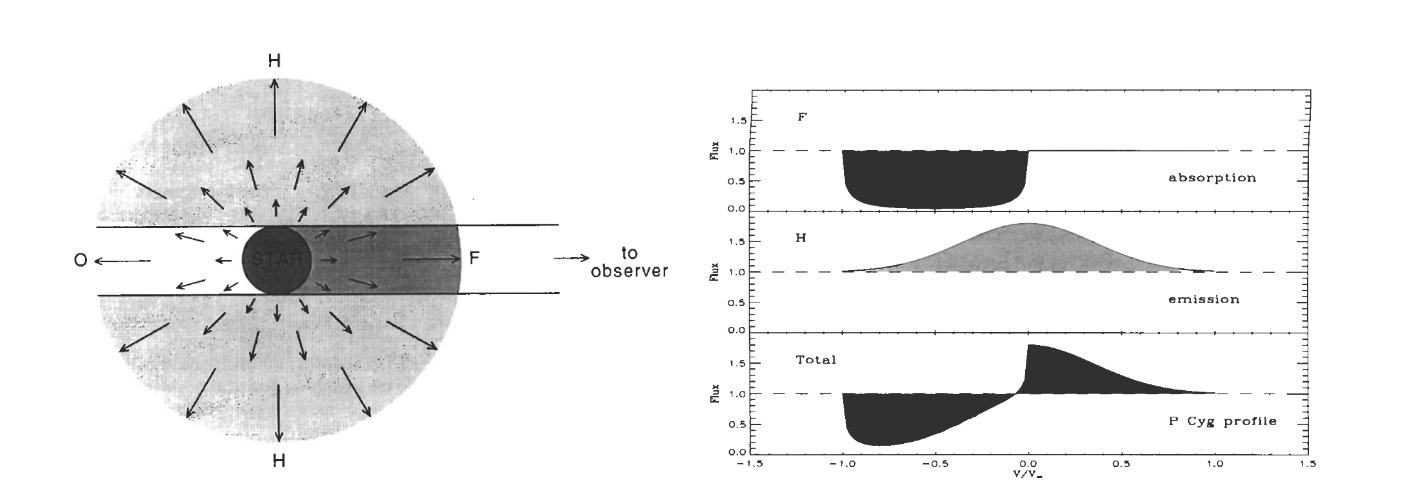
\includegraphics[width=.5\textwidth]{464_p_cygni_profil.png}
  \caption{Das P Cygni Profil eines Sterns. Abzisse: $v/v_\infty$.\cite{anleitung464}} \label{fig:p_cygni_profil}
\end{figure}

Innerhalb des Windes emittiert der Stern Licht.
Dieses Licht wird von dem Sternwind, welcher genau in der Linie zwischen Beobachter und Stern liegt, absorbiert.
Dadurch lässt sich hier eine Verringerung des Flusses feststellen.
Dies erkennt man in Abb.\ (\ref{fig:p_cygni_profil}) in F.
Da sich der Sternwind jenseits des Sterns ausbreitet, wird dort ein größerer Fluss festgestellt, der durch die Emission des Windes selbest hervorgerufen wird.
Dies erkennt man in H.
Hinter dem Stern (relativ zum Beobachter) wird keine Strahlung gemessen, da diese nicht durch den Kern des Sterns zur Seite des Beobachters dringt.
Fügt man F und H zusammen, so ergibt sich eine charakteristische Kurve, die bei Sternen mit Sternwinden auftritt.

Die Absorption ist keine Absorptionslinie, sondern ein Absorptionstrog, da der Sternwind verschiedene Geschwindigkeiten aufweist.
Dabei hat er eine Geschwindigkeit von $-v_\infty$ am äußersten Rand\footnote{Die Bewegung ist relativ zum Beobachter, daher ist die Geschwindigkeit negativ. Die Richtung vom Beobachter weg ist Positiv.} und eine Geschwindigkeit von $v_0\approx v_R$ (die Raidalgeschwindigkeit des Sterns) unmittelbar vor dem Stern. 
%TODO: v_inf näher beschreiben. Was genau meinst du hier mit deine Beschreibung von v_0. Ist das nicht v_0, da die Winde zu uns keien Radialgeschiwndigkeit relativ zum Stern haben? // da hab ich noch nicht über v_R nachgedacht...
Dadurch ist dieser \textsc{Doppler}--verschoben und es bildet sich eine breite Absorptionslinie.

Das Emissionsspektrum ist \textsc{Gauss}--förmig von $-v_\infty$ bis $v_\infty$ da es über den ganzen Umfang des Windes verteilt ist.
Der Emissionspeak ist kreisförmig um den Stern verteilt und besitzt dort -- bei $v\approx 0$ -- ein Maximum.

Die Endwindgeschwindigkeit des Windes kann daher mit dem \textsc{Doppler}--Effekt bestimmt werden, indem die Wellenlängendifferenz der blauen Kante des Absorptionstrogs bei $v=-v_\infty$ und dem Emissionspeak bei $v\approx 0$ verglichen wird.
Dabei ist
\begin{align} 
  \lambda _\text{b}=\lambda _\text{e}\,\sqrt[]{\dfrac{c-v_\infty}{c+v_\infty}}
,\end{align} 
wobei $\lambda _\text{b}$ die Wellenlänge an der blauen Kante des Absorptionstrogs und $\lambda _\text{e}$ der Peak des Emissionsspektrums ist.


\subsection{Durchführung \& Auswertung: P Cygni Profil\\Endsternwindgeschwindigkeit}
Analog zur H$\alpha $ Linie wird das Spektrum von P Cygni aufgenommen, mit nEDAR analysiert und ein linearer Fit zur Wellenlängenkalibrierung durchgeführt.
Da es wie auch in (\ref{sec:beobachtet}) nicht möglich war ein gelungenes Spektrum aufzunehmen, wird hier auf die bereitgestellten Daten zugegriffen.
Hierfür vergleicht man die Analyse des selbst aufgenommenen Spektrums in Abb.\ (\ref{fig:beob_pcygni}) und die des bereitgestellten Spektrums in Abb.\ (\ref{fig:bereit_pcygni}).

Um die Endwindgeschwindigkeit $v_\infty$ zu bestimmen kann wie in \ref{sec:T-H-P-Cygni} vorgegangen werden.
Es ist
\begin{align} 
  v_\infty=\dfrac{c\left(\lambda _\text{e}^2-\lambda _\text{b}^2\right)}{\lambda _\text{e}^2+\lambda _\text{b}^2}
.\end{align} 
Die Wellenlängen $\lambda _\text{e}$ und $\lambda _\text{b}$ werden an dem Plot des P Cygni Profils abgelesen.
Dies wird für die Linien H$\alpha$, N\textsc{ii} $\SI{6482,0}{\r{A}}$ und He\textsc{ii} $\SI{6678,2}{\r{A}}$ durchgeführt.  
Diese sind als gesamtes Spektrum in Abb.\ (\ref{fig:pcygniSpektrum}) und einzeln in (\ref{fig:pcHe2}), (\ref{fig:pcH}), (\ref{fig:pcN2}) und (\ref{fig:pcSi3}) zu sehen.
Die blaue Kannte ist als blaue vertikale Linie eingezeichnet.
Es ergeben sich die Werte aus Tab.\ (\ref{tab:vinf}).
Das Mittel liegt bei
\begin{align} 
  \overline{v_\infty}\approx \SI{1.78+-3366e+5}{m/s}
.\end{align} 
Die Größenordnung ($\approx \SI{178}{km/s}$) liegt im erwarteten Bereich von bis zu $\SI{2000}{km/s}$.
Der relativ große Fehler auf die Endwindgeschwindigkeit der He\textsc{ii} Linie (und damit auch auf den Mittelwert) kommt von den wenigen Datenpunkten, an die eine \textsc{Gauss}--Kurve angepasst werden kann. 


\subsection{Durchführung \& Auswertung: P Cygni Profil\\Radialgeschwindigkeit}
Die Radialgeschwindigkeit des Sterns zum Beobachter kann mit der Rotverschiebung der H$\alpha $ Linie, also dem Emissionspeak des Sternwindes der H$\alpha $ Linie, berechnet werden.
Die \textsc{Doppler}--Verschiebung ergibt sich analog zu (\ref{sec:T-H-P-Cygni}).
Diese ergibt sich dann zu
\begin{align} 
  v_R=-\SI{87325+-2289}{m/s}
.\end{align}
%TODO herleitung v_R (formel) / Gleich wie mit der Blauen Kante. Ist immerhin auch einfach eine Dopplerverschiebung
Der Literaturwert liegt bei\cite{pcygniRadialvelocity}
\begin{align} 
  v_R^\text{lit}=\SI{-8.9}{km/s}
.\end{align} 
%TODO v_inf richtig? / Soll das die Fluchtgeschwindigkeit oder die Radialgeschwindigkeit sein? // lol war falsch
Die Abweichung beträgt ca.\ $38.1\sigma $ bei einem relativen Fehler von 2.6\%. % TODO: der Relative fehler kann nicht stimmen. 2e3 von 8e4 sind nichtmal 10%. // true
Dies ist nicht mit dem Literaturwert vereinbar.
% TODO: das wurde von der Halpha linie abgelesen, bei dem viele Punkte zur verfügung standen. Also das stimmmt so nicht. tbh weiß ich nicht wo der Fehler liegt, da die Daten gut sind und diese Abweichung nicht nur durch schlechtes Fitten oder Abglesen passieren kann. Ich glaube es wäre nochmal gut zu erwähnen, welche daten wir verwednet haben. Es könnte einfach sein, dass wir das falsche Kalibrationsspektrum haben. Unsere Daten sind vom 2021-09-01. Das sind die einzigen Daten von diesem Tag, also sollte es eigentlich keine Verwechslungsgefahr geben. Du kannst die auch nochmal selber auf ecampus angucken. Da würde für unsere Gruppe ein Ordner freigschalten. Da stehen dann auch nochmal die kompletten Namen der Dateien drin. // hab mal die begründung weggemacht. die datei stimmt eig überein.




\section{Fazit}



\bibliography{refs}

\clearpage
\section{Appendix}
\begin{table*}[t]
  \begin{tabular}{cccc}
    \toprule
    & H$\alpha$ & He\textsc{ii} & N\textsc{ii}\\
    \midrule
    $\lambda _\text{b}$ & $\SI{6.5580+-0.0003e-7}{m}$ & $\SI{6.4793+-0.0002e-7}{m}$ & $\SI{6.67404+-0.0004e-7}{m}$ \\
    $\lambda _\text{e}$ & $\SI{6.56272+-0.00005e-7}{m}$ & $\SI{6.482+-21.821e-7}{m}$ & $\SI{6.67807+-0.00009e-7}{m}$ \\
    $v_\infty$ & $\SI{2.1801+-0.1391e+5}{m/s}$ & $\SI{1.36+-10098e+5}{m/s}$ & $\SI{1.808+-0.201e+5}{m/s}$ \\
    \bottomrule
  \end{tabular}
  \caption{Die Endwindgeschwindigkeiten der verschiedenen Emissionslinien.} \label{tab:vinf}
\end{table*}
% zuordnung:
% n: stern
% a: spektrum
% b: anpassung Ha
% c: kalibrierung
\begin{figure}[h]
  \centering
  \resizebox{.5\textwidth}{!}{% GNUPLOT: LaTeX picture with Postscript
\begingroup
  \makeatletter
  \providecommand\color[2][]{%
    \GenericError{(gnuplot) \space\space\space\@spaces}{%
      Package color not loaded in conjunction with
      terminal option `colourtext'%
    }{See the gnuplot documentation for explanation.%
    }{Either use 'blacktext' in gnuplot or load the package
      color.sty in LaTeX.}%
    \renewcommand\color[2][]{}%
  }%
  \providecommand\includegraphics[2][]{%
    \GenericError{(gnuplot) \space\space\space\@spaces}{%
      Package graphicx or graphics not loaded%
    }{See the gnuplot documentation for explanation.%
    }{The gnuplot epslatex terminal needs graphicx.sty or graphics.sty.}%
    \renewcommand\includegraphics[2][]{}%
  }%
  \providecommand\rotatebox[2]{#2}%
  \@ifundefined{ifGPcolor}{%
    \newif\ifGPcolor
    \GPcolortrue
  }{}%
  \@ifundefined{ifGPblacktext}{%
    \newif\ifGPblacktext
    \GPblacktexttrue
  }{}%
  % define a \g@addto@macro without @ in the name:
  \let\gplgaddtomacro\g@addto@macro
  % define empty templates for all commands taking text:
  \gdef\gplbacktext{}%
  \gdef\gplfronttext{}%
  \makeatother
  \ifGPblacktext
    % no textcolor at all
    \def\colorrgb#1{}%
    \def\colorgray#1{}%
  \else
    % gray or color?
    \ifGPcolor
      \def\colorrgb#1{\color[rgb]{#1}}%
      \def\colorgray#1{\color[gray]{#1}}%
      \expandafter\def\csname LTw\endcsname{\color{white}}%
      \expandafter\def\csname LTb\endcsname{\color{black}}%
      \expandafter\def\csname LTa\endcsname{\color{black}}%
      \expandafter\def\csname LT0\endcsname{\color[rgb]{1,0,0}}%
      \expandafter\def\csname LT1\endcsname{\color[rgb]{0,1,0}}%
      \expandafter\def\csname LT2\endcsname{\color[rgb]{0,0,1}}%
      \expandafter\def\csname LT3\endcsname{\color[rgb]{1,0,1}}%
      \expandafter\def\csname LT4\endcsname{\color[rgb]{0,1,1}}%
      \expandafter\def\csname LT5\endcsname{\color[rgb]{1,1,0}}%
      \expandafter\def\csname LT6\endcsname{\color[rgb]{0,0,0}}%
      \expandafter\def\csname LT7\endcsname{\color[rgb]{1,0.3,0}}%
      \expandafter\def\csname LT8\endcsname{\color[rgb]{0.5,0.5,0.5}}%
    \else
      % gray
      \def\colorrgb#1{\color{black}}%
      \def\colorgray#1{\color[gray]{#1}}%
      \expandafter\def\csname LTw\endcsname{\color{white}}%
      \expandafter\def\csname LTb\endcsname{\color{black}}%
      \expandafter\def\csname LTa\endcsname{\color{black}}%
      \expandafter\def\csname LT0\endcsname{\color{black}}%
      \expandafter\def\csname LT1\endcsname{\color{black}}%
      \expandafter\def\csname LT2\endcsname{\color{black}}%
      \expandafter\def\csname LT3\endcsname{\color{black}}%
      \expandafter\def\csname LT4\endcsname{\color{black}}%
      \expandafter\def\csname LT5\endcsname{\color{black}}%
      \expandafter\def\csname LT6\endcsname{\color{black}}%
      \expandafter\def\csname LT7\endcsname{\color{black}}%
      \expandafter\def\csname LT8\endcsname{\color{black}}%
    \fi
  \fi
    \setlength{\unitlength}{0.0500bp}%
    \ifx\gptboxheight\undefined%
      \newlength{\gptboxheight}%
      \newlength{\gptboxwidth}%
      \newsavebox{\gptboxtext}%
    \fi%
    \setlength{\fboxrule}{0.5pt}%
    \setlength{\fboxsep}{1pt}%
    \definecolor{tbcol}{rgb}{1,1,1}%
\begin{picture}(7200.00,4320.00)%
    \gplgaddtomacro\gplbacktext{%
      \csname LTb\endcsname%%
      \put(1123,619){\makebox(0,0)[r]{\strut{}200\cdot10^{-3}}}%
      \csname LTb\endcsname%%
      \put(1123,1006){\makebox(0,0)[r]{\strut{}300\cdot10^{-3}}}%
      \csname LTb\endcsname%%
      \put(1123,1394){\makebox(0,0)[r]{\strut{}400\cdot10^{-3}}}%
      \csname LTb\endcsname%%
      \put(1123,1781){\makebox(0,0)[r]{\strut{}500\cdot10^{-3}}}%
      \csname LTb\endcsname%%
      \put(1123,2169){\makebox(0,0)[r]{\strut{}600\cdot10^{-3}}}%
      \csname LTb\endcsname%%
      \put(1123,2556){\makebox(0,0)[r]{\strut{}700\cdot10^{-3}}}%
      \csname LTb\endcsname%%
      \put(1123,2944){\makebox(0,0)[r]{\strut{}800\cdot10^{-3}}}%
      \csname LTb\endcsname%%
      \put(1123,3331){\makebox(0,0)[r]{\strut{}900\cdot10^{-3}}}%
      \csname LTb\endcsname%%
      \put(1123,3719){\makebox(0,0)[r]{\strut{}1\cdot10^{0}}}%
      \csname LTb\endcsname%%
      \put(1221,425){\makebox(0,0){\strut{}$0$}}%
      \csname LTb\endcsname%%
      \put(1929,425){\makebox(0,0){\strut{}$100$}}%
      \csname LTb\endcsname%%
      \put(2637,425){\makebox(0,0){\strut{}$200$}}%
      \csname LTb\endcsname%%
      \put(3345,425){\makebox(0,0){\strut{}$300$}}%
      \csname LTb\endcsname%%
      \put(4053,425){\makebox(0,0){\strut{}$400$}}%
      \csname LTb\endcsname%%
      \put(4761,425){\makebox(0,0){\strut{}$500$}}%
      \csname LTb\endcsname%%
      \put(5470,425){\makebox(0,0){\strut{}$600$}}%
      \csname LTb\endcsname%%
      \put(6178,425){\makebox(0,0){\strut{}$700$}}%
      \csname LTb\endcsname%%
      \put(6886,425){\makebox(0,0){\strut{}$800$}}%
    }%
    \gplgaddtomacro\gplfronttext{%
      \csname LTb\endcsname%%
      \put(6123,3545){\makebox(0,0)[r]{\strut{}109358-G0}}%
      \csname LTb\endcsname%%
      \put(6123,3351){\makebox(0,0)[r]{\strut{}Kalibrationslampe}}%
      \csname LTb\endcsname%%
      \put(170,2169){\rotatebox{-270.00}{\makebox(0,0){\strut{}Amplitude$/\textrm{a.u.}$}}}%
      \csname LTb\endcsname%%
      \put(4053,135){\makebox(0,0){\strut{}Pixelkoordinate$/\textrm{Pixel}$}}%
      \csname LTb\endcsname%%
      \put(4053,4009){\makebox(0,0){\strut{}Spektrum}}%
    }%
    \gplbacktext
    \put(0,0){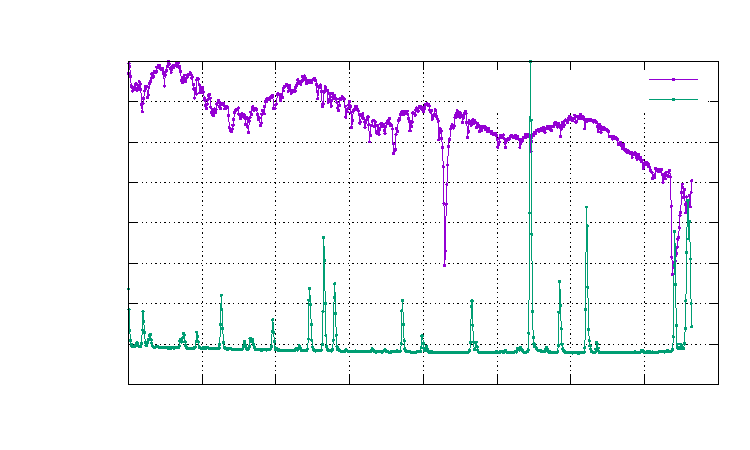
\includegraphics[width={360.00bp},height={216.00bp}]{109358-G0_data}}%
    \gplfronttext
  \end{picture}%
\endgroup
}
  \caption{} \label{fig:1a}
\end{figure}
\begin{figure}[h]
  \centering
  \resizebox{.5\textwidth}{!}{% GNUPLOT: LaTeX picture with Postscript
\begingroup
  \makeatletter
  \providecommand\color[2][]{%
    \GenericError{(gnuplot) \space\space\space\@spaces}{%
      Package color not loaded in conjunction with
      terminal option `colourtext'%
    }{See the gnuplot documentation for explanation.%
    }{Either use 'blacktext' in gnuplot or load the package
      color.sty in LaTeX.}%
    \renewcommand\color[2][]{}%
  }%
  \providecommand\includegraphics[2][]{%
    \GenericError{(gnuplot) \space\space\space\@spaces}{%
      Package graphicx or graphics not loaded%
    }{See the gnuplot documentation for explanation.%
    }{The gnuplot epslatex terminal needs graphicx.sty or graphics.sty.}%
    \renewcommand\includegraphics[2][]{}%
  }%
  \providecommand\rotatebox[2]{#2}%
  \@ifundefined{ifGPcolor}{%
    \newif\ifGPcolor
    \GPcolortrue
  }{}%
  \@ifundefined{ifGPblacktext}{%
    \newif\ifGPblacktext
    \GPblacktexttrue
  }{}%
  % define a \g@addto@macro without @ in the name:
  \let\gplgaddtomacro\g@addto@macro
  % define empty templates for all commands taking text:
  \gdef\gplbacktext{}%
  \gdef\gplfronttext{}%
  \makeatother
  \ifGPblacktext
    % no textcolor at all
    \def\colorrgb#1{}%
    \def\colorgray#1{}%
  \else
    % gray or color?
    \ifGPcolor
      \def\colorrgb#1{\color[rgb]{#1}}%
      \def\colorgray#1{\color[gray]{#1}}%
      \expandafter\def\csname LTw\endcsname{\color{white}}%
      \expandafter\def\csname LTb\endcsname{\color{black}}%
      \expandafter\def\csname LTa\endcsname{\color{black}}%
      \expandafter\def\csname LT0\endcsname{\color[rgb]{1,0,0}}%
      \expandafter\def\csname LT1\endcsname{\color[rgb]{0,1,0}}%
      \expandafter\def\csname LT2\endcsname{\color[rgb]{0,0,1}}%
      \expandafter\def\csname LT3\endcsname{\color[rgb]{1,0,1}}%
      \expandafter\def\csname LT4\endcsname{\color[rgb]{0,1,1}}%
      \expandafter\def\csname LT5\endcsname{\color[rgb]{1,1,0}}%
      \expandafter\def\csname LT6\endcsname{\color[rgb]{0,0,0}}%
      \expandafter\def\csname LT7\endcsname{\color[rgb]{1,0.3,0}}%
      \expandafter\def\csname LT8\endcsname{\color[rgb]{0.5,0.5,0.5}}%
    \else
      % gray
      \def\colorrgb#1{\color{black}}%
      \def\colorgray#1{\color[gray]{#1}}%
      \expandafter\def\csname LTw\endcsname{\color{white}}%
      \expandafter\def\csname LTb\endcsname{\color{black}}%
      \expandafter\def\csname LTa\endcsname{\color{black}}%
      \expandafter\def\csname LT0\endcsname{\color{black}}%
      \expandafter\def\csname LT1\endcsname{\color{black}}%
      \expandafter\def\csname LT2\endcsname{\color{black}}%
      \expandafter\def\csname LT3\endcsname{\color{black}}%
      \expandafter\def\csname LT4\endcsname{\color{black}}%
      \expandafter\def\csname LT5\endcsname{\color{black}}%
      \expandafter\def\csname LT6\endcsname{\color{black}}%
      \expandafter\def\csname LT7\endcsname{\color{black}}%
      \expandafter\def\csname LT8\endcsname{\color{black}}%
    \fi
  \fi
    \setlength{\unitlength}{0.0500bp}%
    \ifx\gptboxheight\undefined%
      \newlength{\gptboxheight}%
      \newlength{\gptboxwidth}%
      \newsavebox{\gptboxtext}%
    \fi%
    \setlength{\fboxrule}{0.5pt}%
    \setlength{\fboxsep}{1pt}%
    \definecolor{tbcol}{rgb}{1,1,1}%
\begin{picture}(7200.00,4320.00)%
    \gplgaddtomacro\gplbacktext{%
      \csname LTb\endcsname%%
      \put(1025,619){\makebox(0,0)[r]{\strut{}$70\cdot10^{3}$}}%
      \csname LTb\endcsname%%
      \put(1025,1062){\makebox(0,0)[r]{\strut{}$80\cdot10^{3}$}}%
      \csname LTb\endcsname%%
      \put(1025,1505){\makebox(0,0)[r]{\strut{}$90\cdot10^{3}$}}%
      \csname LTb\endcsname%%
      \put(1025,1947){\makebox(0,0)[r]{\strut{}$100\cdot10^{3}$}}%
      \csname LTb\endcsname%%
      \put(1025,2390){\makebox(0,0)[r]{\strut{}$110\cdot10^{3}$}}%
      \csname LTb\endcsname%%
      \put(1025,2833){\makebox(0,0)[r]{\strut{}$120\cdot10^{3}$}}%
      \csname LTb\endcsname%%
      \put(1025,3276){\makebox(0,0)[r]{\strut{}$130\cdot10^{3}$}}%
      \csname LTb\endcsname%%
      \put(1025,3719){\makebox(0,0)[r]{\strut{}$140\cdot10^{3}$}}%
      \csname LTb\endcsname%%
      \put(2276,425){\makebox(0,0){\strut{}$650\cdot10^{-9}$}}%
      \csname LTb\endcsname%%
      \put(3716,425){\makebox(0,0){\strut{}$655\cdot10^{-9}$}}%
      \csname LTb\endcsname%%
      \put(5157,425){\makebox(0,0){\strut{}$660\cdot10^{-9}$}}%
      \csname LTb\endcsname%%
      \put(6598,425){\makebox(0,0){\strut{}$665\cdot10^{-9}$}}%
    }%
    \gplgaddtomacro\gplfronttext{%
      \csname LTb\endcsname%%
      \put(170,2169){\rotatebox{-270}{\makebox(0,0){\strut{}Amplitude$/\textrm{a.u.}$}}}%
      \csname LTb\endcsname%%
      \put(4004,135){\makebox(0,0){\strut{}Wellenlänge $\lambda/\SI{}{m}$}}%
      \csname LTb\endcsname%%
      \put(6123,986){\makebox(0,0)[r]{\strut{}Datenpunkte}}%
      \csname LTb\endcsname%%
      \put(6123,793){\makebox(0,0)[r]{\strut{}Anpassung $G_\text{f}(x)$}}%
      \csname LTb\endcsname%%
      \put(4004,4009){\makebox(0,0){\strut{}H$\alpha$(\SI{656}{nm})-Linie von 109358-G0 mit $\chi^2/\textrm{ddof}=\SI{1.16E+01}{}$}}%
    }%
    \gplbacktext
    \put(0,0){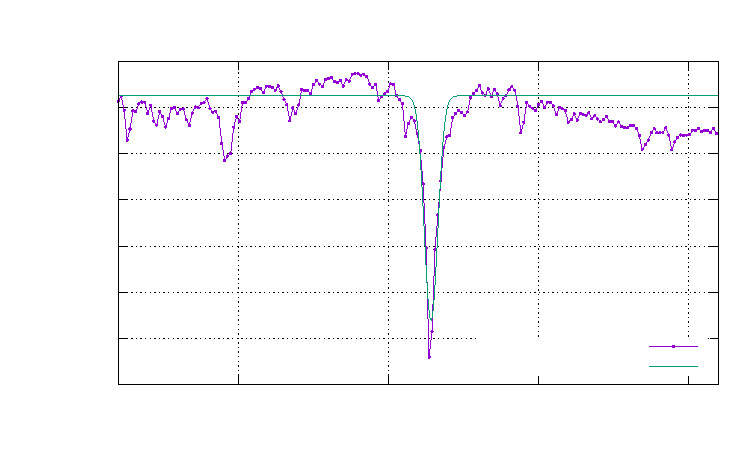
\includegraphics[width={360.00bp},height={216.00bp}]{109358-G0_gauss}}%
    \gplfronttext
  \end{picture}%
\endgroup
}
  \caption{} \label{fig:1b}
\end{figure}
\begin{figure}[h]
  \centering
  \resizebox{.5\textwidth}{!}{% GNUPLOT: LaTeX picture with Postscript
\begingroup
  \makeatletter
  \providecommand\color[2][]{%
    \GenericError{(gnuplot) \space\space\space\@spaces}{%
      Package color not loaded in conjunction with
      terminal option `colourtext'%
    }{See the gnuplot documentation for explanation.%
    }{Either use 'blacktext' in gnuplot or load the package
      color.sty in LaTeX.}%
    \renewcommand\color[2][]{}%
  }%
  \providecommand\includegraphics[2][]{%
    \GenericError{(gnuplot) \space\space\space\@spaces}{%
      Package graphicx or graphics not loaded%
    }{See the gnuplot documentation for explanation.%
    }{The gnuplot epslatex terminal needs graphicx.sty or graphics.sty.}%
    \renewcommand\includegraphics[2][]{}%
  }%
  \providecommand\rotatebox[2]{#2}%
  \@ifundefined{ifGPcolor}{%
    \newif\ifGPcolor
    \GPcolortrue
  }{}%
  \@ifundefined{ifGPblacktext}{%
    \newif\ifGPblacktext
    \GPblacktexttrue
  }{}%
  % define a \g@addto@macro without @ in the name:
  \let\gplgaddtomacro\g@addto@macro
  % define empty templates for all commands taking text:
  \gdef\gplbacktext{}%
  \gdef\gplfronttext{}%
  \makeatother
  \ifGPblacktext
    % no textcolor at all
    \def\colorrgb#1{}%
    \def\colorgray#1{}%
  \else
    % gray or color?
    \ifGPcolor
      \def\colorrgb#1{\color[rgb]{#1}}%
      \def\colorgray#1{\color[gray]{#1}}%
      \expandafter\def\csname LTw\endcsname{\color{white}}%
      \expandafter\def\csname LTb\endcsname{\color{black}}%
      \expandafter\def\csname LTa\endcsname{\color{black}}%
      \expandafter\def\csname LT0\endcsname{\color[rgb]{1,0,0}}%
      \expandafter\def\csname LT1\endcsname{\color[rgb]{0,1,0}}%
      \expandafter\def\csname LT2\endcsname{\color[rgb]{0,0,1}}%
      \expandafter\def\csname LT3\endcsname{\color[rgb]{1,0,1}}%
      \expandafter\def\csname LT4\endcsname{\color[rgb]{0,1,1}}%
      \expandafter\def\csname LT5\endcsname{\color[rgb]{1,1,0}}%
      \expandafter\def\csname LT6\endcsname{\color[rgb]{0,0,0}}%
      \expandafter\def\csname LT7\endcsname{\color[rgb]{1,0.3,0}}%
      \expandafter\def\csname LT8\endcsname{\color[rgb]{0.5,0.5,0.5}}%
    \else
      % gray
      \def\colorrgb#1{\color{black}}%
      \def\colorgray#1{\color[gray]{#1}}%
      \expandafter\def\csname LTw\endcsname{\color{white}}%
      \expandafter\def\csname LTb\endcsname{\color{black}}%
      \expandafter\def\csname LTa\endcsname{\color{black}}%
      \expandafter\def\csname LT0\endcsname{\color{black}}%
      \expandafter\def\csname LT1\endcsname{\color{black}}%
      \expandafter\def\csname LT2\endcsname{\color{black}}%
      \expandafter\def\csname LT3\endcsname{\color{black}}%
      \expandafter\def\csname LT4\endcsname{\color{black}}%
      \expandafter\def\csname LT5\endcsname{\color{black}}%
      \expandafter\def\csname LT6\endcsname{\color{black}}%
      \expandafter\def\csname LT7\endcsname{\color{black}}%
      \expandafter\def\csname LT8\endcsname{\color{black}}%
    \fi
  \fi
    \setlength{\unitlength}{0.0500bp}%
    \ifx\gptboxheight\undefined%
      \newlength{\gptboxheight}%
      \newlength{\gptboxwidth}%
      \newsavebox{\gptboxtext}%
    \fi%
    \setlength{\fboxrule}{0.5pt}%
    \setlength{\fboxsep}{1pt}%
    \definecolor{tbcol}{rgb}{1,1,1}%
\begin{picture}(7200.00,4320.00)%
    \gplgaddtomacro\gplbacktext{%
      \csname LTb\endcsname%%
      \put(1123,619){\makebox(0,0)[r]{\strut{}635\cdot10^{-9}}}%
      \csname LTb\endcsname%%
      \put(1123,963){\makebox(0,0)[r]{\strut{}640\cdot10^{-9}}}%
      \csname LTb\endcsname%%
      \put(1123,1308){\makebox(0,0)[r]{\strut{}645\cdot10^{-9}}}%
      \csname LTb\endcsname%%
      \put(1123,1652){\makebox(0,0)[r]{\strut{}650\cdot10^{-9}}}%
      \csname LTb\endcsname%%
      \put(1123,1997){\makebox(0,0)[r]{\strut{}655\cdot10^{-9}}}%
      \csname LTb\endcsname%%
      \put(1123,2341){\makebox(0,0)[r]{\strut{}660\cdot10^{-9}}}%
      \csname LTb\endcsname%%
      \put(1123,2686){\makebox(0,0)[r]{\strut{}665\cdot10^{-9}}}%
      \csname LTb\endcsname%%
      \put(1123,3030){\makebox(0,0)[r]{\strut{}670\cdot10^{-9}}}%
      \csname LTb\endcsname%%
      \put(1123,3374){\makebox(0,0)[r]{\strut{}675\cdot10^{-9}}}%
      \csname LTb\endcsname%%
      \put(1123,3719){\makebox(0,0)[r]{\strut{}680\cdot10^{-9}}}%
      \csname LTb\endcsname%%
      \put(1221,425){\makebox(0,0){\strut{}$200$}}%
      \csname LTb\endcsname%%
      \put(1850,425){\makebox(0,0){\strut{}$250$}}%
      \csname LTb\endcsname%%
      \put(2480,425){\makebox(0,0){\strut{}$300$}}%
      \csname LTb\endcsname%%
      \put(3109,425){\makebox(0,0){\strut{}$350$}}%
      \csname LTb\endcsname%%
      \put(3739,425){\makebox(0,0){\strut{}$400$}}%
      \csname LTb\endcsname%%
      \put(4368,425){\makebox(0,0){\strut{}$450$}}%
      \csname LTb\endcsname%%
      \put(4997,425){\makebox(0,0){\strut{}$500$}}%
      \csname LTb\endcsname%%
      \put(5627,425){\makebox(0,0){\strut{}$550$}}%
      \csname LTb\endcsname%%
      \put(6256,425){\makebox(0,0){\strut{}$600$}}%
      \csname LTb\endcsname%%
      \put(6886,425){\makebox(0,0){\strut{}$650$}}%
    }%
    \gplgaddtomacro\gplfronttext{%
      \csname LTb\endcsname%%
      \put(6123,3545){\makebox(0,0)[r]{\strut{}Datenpunkte}}%
      \csname LTb\endcsname%%
      \put(6123,3351){\makebox(0,0)[r]{\strut{}Anpassung $\lambda_\text{f}(x)$}}%
      \csname LTb\endcsname%%
      \put(170,2169){\rotatebox{-270.00}{\makebox(0,0){\strut{}Wellenlänge $\lambda/\SI{}{m}$}}}%
      \csname LTb\endcsname%%
      \put(4053,135){\makebox(0,0){\strut{}Pixelkoordinate$/\textrm{Pixel}$}}%
      \csname LTb\endcsname%%
      \put(4053,4009){\makebox(0,0){\strut{}Kalibraiton des 109358-G0 Spektrums mit $\chi^2/\textrm{ddof}=\SI{3.03E-02}{}$}}%
    }%
    \gplbacktext
    \put(0,0){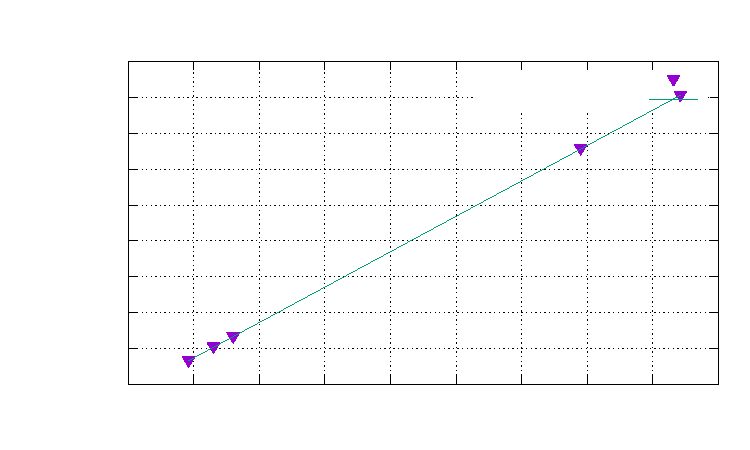
\includegraphics[width={360.00bp},height={216.00bp}]{109358-G0_kali}}%
    \gplfronttext
  \end{picture}%
\endgroup
}
  \caption{} \label{fig:1c}
\end{figure}
\begin{figure}[h]
  \centering
  \resizebox{.5\textwidth}{!}{% GNUPLOT: LaTeX picture with Postscript
\begingroup
  \makeatletter
  \providecommand\color[2][]{%
    \GenericError{(gnuplot) \space\space\space\@spaces}{%
      Package color not loaded in conjunction with
      terminal option `colourtext'%
    }{See the gnuplot documentation for explanation.%
    }{Either use 'blacktext' in gnuplot or load the package
      color.sty in LaTeX.}%
    \renewcommand\color[2][]{}%
  }%
  \providecommand\includegraphics[2][]{%
    \GenericError{(gnuplot) \space\space\space\@spaces}{%
      Package graphicx or graphics not loaded%
    }{See the gnuplot documentation for explanation.%
    }{The gnuplot epslatex terminal needs graphicx.sty or graphics.sty.}%
    \renewcommand\includegraphics[2][]{}%
  }%
  \providecommand\rotatebox[2]{#2}%
  \@ifundefined{ifGPcolor}{%
    \newif\ifGPcolor
    \GPcolortrue
  }{}%
  \@ifundefined{ifGPblacktext}{%
    \newif\ifGPblacktext
    \GPblacktexttrue
  }{}%
  % define a \g@addto@macro without @ in the name:
  \let\gplgaddtomacro\g@addto@macro
  % define empty templates for all commands taking text:
  \gdef\gplbacktext{}%
  \gdef\gplfronttext{}%
  \makeatother
  \ifGPblacktext
    % no textcolor at all
    \def\colorrgb#1{}%
    \def\colorgray#1{}%
  \else
    % gray or color?
    \ifGPcolor
      \def\colorrgb#1{\color[rgb]{#1}}%
      \def\colorgray#1{\color[gray]{#1}}%
      \expandafter\def\csname LTw\endcsname{\color{white}}%
      \expandafter\def\csname LTb\endcsname{\color{black}}%
      \expandafter\def\csname LTa\endcsname{\color{black}}%
      \expandafter\def\csname LT0\endcsname{\color[rgb]{1,0,0}}%
      \expandafter\def\csname LT1\endcsname{\color[rgb]{0,1,0}}%
      \expandafter\def\csname LT2\endcsname{\color[rgb]{0,0,1}}%
      \expandafter\def\csname LT3\endcsname{\color[rgb]{1,0,1}}%
      \expandafter\def\csname LT4\endcsname{\color[rgb]{0,1,1}}%
      \expandafter\def\csname LT5\endcsname{\color[rgb]{1,1,0}}%
      \expandafter\def\csname LT6\endcsname{\color[rgb]{0,0,0}}%
      \expandafter\def\csname LT7\endcsname{\color[rgb]{1,0.3,0}}%
      \expandafter\def\csname LT8\endcsname{\color[rgb]{0.5,0.5,0.5}}%
    \else
      % gray
      \def\colorrgb#1{\color{black}}%
      \def\colorgray#1{\color[gray]{#1}}%
      \expandafter\def\csname LTw\endcsname{\color{white}}%
      \expandafter\def\csname LTb\endcsname{\color{black}}%
      \expandafter\def\csname LTa\endcsname{\color{black}}%
      \expandafter\def\csname LT0\endcsname{\color{black}}%
      \expandafter\def\csname LT1\endcsname{\color{black}}%
      \expandafter\def\csname LT2\endcsname{\color{black}}%
      \expandafter\def\csname LT3\endcsname{\color{black}}%
      \expandafter\def\csname LT4\endcsname{\color{black}}%
      \expandafter\def\csname LT5\endcsname{\color{black}}%
      \expandafter\def\csname LT6\endcsname{\color{black}}%
      \expandafter\def\csname LT7\endcsname{\color{black}}%
      \expandafter\def\csname LT8\endcsname{\color{black}}%
    \fi
  \fi
    \setlength{\unitlength}{0.0500bp}%
    \ifx\gptboxheight\undefined%
      \newlength{\gptboxheight}%
      \newlength{\gptboxwidth}%
      \newsavebox{\gptboxtext}%
    \fi%
    \setlength{\fboxrule}{0.5pt}%
    \setlength{\fboxsep}{1pt}%
    \definecolor{tbcol}{rgb}{1,1,1}%
\begin{picture}(7200.00,4320.00)%
    \gplgaddtomacro\gplbacktext{%
      \csname LTb\endcsname%%
      \put(1123,619){\makebox(0,0)[r]{\strut{}$200\cdot10^{-3}$}}%
      \csname LTb\endcsname%%
      \put(1123,1006){\makebox(0,0)[r]{\strut{}$300\cdot10^{-3}$}}%
      \csname LTb\endcsname%%
      \put(1123,1394){\makebox(0,0)[r]{\strut{}$400\cdot10^{-3}$}}%
      \csname LTb\endcsname%%
      \put(1123,1781){\makebox(0,0)[r]{\strut{}$500\cdot10^{-3}$}}%
      \csname LTb\endcsname%%
      \put(1123,2169){\makebox(0,0)[r]{\strut{}$600\cdot10^{-3}$}}%
      \csname LTb\endcsname%%
      \put(1123,2556){\makebox(0,0)[r]{\strut{}$700\cdot10^{-3}$}}%
      \csname LTb\endcsname%%
      \put(1123,2944){\makebox(0,0)[r]{\strut{}$800\cdot10^{-3}$}}%
      \csname LTb\endcsname%%
      \put(1123,3331){\makebox(0,0)[r]{\strut{}$900\cdot10^{-3}$}}%
      \csname LTb\endcsname%%
      \put(1123,3719){\makebox(0,0)[r]{\strut{}$1\cdot10^{0}$}}%
      \csname LTb\endcsname%%
      \put(1221,425){\makebox(0,0){\strut{}$0$}}%
      \csname LTb\endcsname%%
      \put(1929,425){\makebox(0,0){\strut{}$100$}}%
      \csname LTb\endcsname%%
      \put(2637,425){\makebox(0,0){\strut{}$200$}}%
      \csname LTb\endcsname%%
      \put(3345,425){\makebox(0,0){\strut{}$300$}}%
      \csname LTb\endcsname%%
      \put(4053,425){\makebox(0,0){\strut{}$400$}}%
      \csname LTb\endcsname%%
      \put(4761,425){\makebox(0,0){\strut{}$500$}}%
      \csname LTb\endcsname%%
      \put(5470,425){\makebox(0,0){\strut{}$600$}}%
      \csname LTb\endcsname%%
      \put(6178,425){\makebox(0,0){\strut{}$700$}}%
      \csname LTb\endcsname%%
      \put(6886,425){\makebox(0,0){\strut{}$800$}}%
    }%
    \gplgaddtomacro\gplfronttext{%
      \csname LTb\endcsname%%
      \put(170,2169){\rotatebox{-270}{\makebox(0,0){\strut{}Amplitude$/\textrm{a.u.}$}}}%
      \csname LTb\endcsname%%
      \put(4053,135){\makebox(0,0){\strut{}Pixelkoordinate$/\textrm{Pixel}$}}%
      \csname LTb\endcsname%%
      \put(6123,3545){\makebox(0,0)[r]{\strut{}134083-F5}}%
      \csname LTb\endcsname%%
      \put(6123,3351){\makebox(0,0)[r]{\strut{}Kalibrationslampe}}%
      \csname LTb\endcsname%%
      \put(4053,4009){\makebox(0,0){\strut{}Spektrum}}%
    }%
    \gplbacktext
    \put(0,0){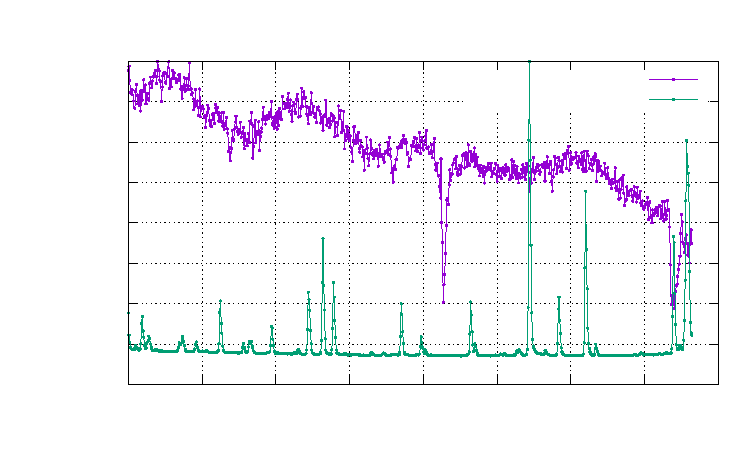
\includegraphics[width={360.00bp},height={216.00bp}]{134083-F5_data}}%
    \gplfronttext
  \end{picture}%
\endgroup
}
  \caption{} \label{fig:2a}
\end{figure}
\begin{figure}[h]
  \centering
  \resizebox{.5\textwidth}{!}{% GNUPLOT: LaTeX picture with Postscript
\begingroup
  \makeatletter
  \providecommand\color[2][]{%
    \GenericError{(gnuplot) \space\space\space\@spaces}{%
      Package color not loaded in conjunction with
      terminal option `colourtext'%
    }{See the gnuplot documentation for explanation.%
    }{Either use 'blacktext' in gnuplot or load the package
      color.sty in LaTeX.}%
    \renewcommand\color[2][]{}%
  }%
  \providecommand\includegraphics[2][]{%
    \GenericError{(gnuplot) \space\space\space\@spaces}{%
      Package graphicx or graphics not loaded%
    }{See the gnuplot documentation for explanation.%
    }{The gnuplot epslatex terminal needs graphicx.sty or graphics.sty.}%
    \renewcommand\includegraphics[2][]{}%
  }%
  \providecommand\rotatebox[2]{#2}%
  \@ifundefined{ifGPcolor}{%
    \newif\ifGPcolor
    \GPcolortrue
  }{}%
  \@ifundefined{ifGPblacktext}{%
    \newif\ifGPblacktext
    \GPblacktexttrue
  }{}%
  % define a \g@addto@macro without @ in the name:
  \let\gplgaddtomacro\g@addto@macro
  % define empty templates for all commands taking text:
  \gdef\gplbacktext{}%
  \gdef\gplfronttext{}%
  \makeatother
  \ifGPblacktext
    % no textcolor at all
    \def\colorrgb#1{}%
    \def\colorgray#1{}%
  \else
    % gray or color?
    \ifGPcolor
      \def\colorrgb#1{\color[rgb]{#1}}%
      \def\colorgray#1{\color[gray]{#1}}%
      \expandafter\def\csname LTw\endcsname{\color{white}}%
      \expandafter\def\csname LTb\endcsname{\color{black}}%
      \expandafter\def\csname LTa\endcsname{\color{black}}%
      \expandafter\def\csname LT0\endcsname{\color[rgb]{1,0,0}}%
      \expandafter\def\csname LT1\endcsname{\color[rgb]{0,1,0}}%
      \expandafter\def\csname LT2\endcsname{\color[rgb]{0,0,1}}%
      \expandafter\def\csname LT3\endcsname{\color[rgb]{1,0,1}}%
      \expandafter\def\csname LT4\endcsname{\color[rgb]{0,1,1}}%
      \expandafter\def\csname LT5\endcsname{\color[rgb]{1,1,0}}%
      \expandafter\def\csname LT6\endcsname{\color[rgb]{0,0,0}}%
      \expandafter\def\csname LT7\endcsname{\color[rgb]{1,0.3,0}}%
      \expandafter\def\csname LT8\endcsname{\color[rgb]{0.5,0.5,0.5}}%
    \else
      % gray
      \def\colorrgb#1{\color{black}}%
      \def\colorgray#1{\color[gray]{#1}}%
      \expandafter\def\csname LTw\endcsname{\color{white}}%
      \expandafter\def\csname LTb\endcsname{\color{black}}%
      \expandafter\def\csname LTa\endcsname{\color{black}}%
      \expandafter\def\csname LT0\endcsname{\color{black}}%
      \expandafter\def\csname LT1\endcsname{\color{black}}%
      \expandafter\def\csname LT2\endcsname{\color{black}}%
      \expandafter\def\csname LT3\endcsname{\color{black}}%
      \expandafter\def\csname LT4\endcsname{\color{black}}%
      \expandafter\def\csname LT5\endcsname{\color{black}}%
      \expandafter\def\csname LT6\endcsname{\color{black}}%
      \expandafter\def\csname LT7\endcsname{\color{black}}%
      \expandafter\def\csname LT8\endcsname{\color{black}}%
    \fi
  \fi
    \setlength{\unitlength}{0.0500bp}%
    \ifx\gptboxheight\undefined%
      \newlength{\gptboxheight}%
      \newlength{\gptboxwidth}%
      \newsavebox{\gptboxtext}%
    \fi%
    \setlength{\fboxrule}{0.5pt}%
    \setlength{\fboxsep}{1pt}%
    \definecolor{tbcol}{rgb}{1,1,1}%
\begin{picture}(7200.00,4320.00)%
    \gplgaddtomacro\gplbacktext{%
      \csname LTb\endcsname%%
      \put(927,619){\makebox(0,0)[r]{\strut{}$9\cdot10^{3}$}}%
      \csname LTb\endcsname%%
      \put(927,929){\makebox(0,0)[r]{\strut{}$10\cdot10^{3}$}}%
      \csname LTb\endcsname%%
      \put(927,1239){\makebox(0,0)[r]{\strut{}$11\cdot10^{3}$}}%
      \csname LTb\endcsname%%
      \put(927,1549){\makebox(0,0)[r]{\strut{}$12\cdot10^{3}$}}%
      \csname LTb\endcsname%%
      \put(927,1859){\makebox(0,0)[r]{\strut{}$13\cdot10^{3}$}}%
      \csname LTb\endcsname%%
      \put(927,2169){\makebox(0,0)[r]{\strut{}$14\cdot10^{3}$}}%
      \csname LTb\endcsname%%
      \put(927,2479){\makebox(0,0)[r]{\strut{}$15\cdot10^{3}$}}%
      \csname LTb\endcsname%%
      \put(927,2789){\makebox(0,0)[r]{\strut{}$16\cdot10^{3}$}}%
      \csname LTb\endcsname%%
      \put(927,3099){\makebox(0,0)[r]{\strut{}$17\cdot10^{3}$}}%
      \csname LTb\endcsname%%
      \put(927,3409){\makebox(0,0)[r]{\strut{}$18\cdot10^{3}$}}%
      \csname LTb\endcsname%%
      \put(927,3719){\makebox(0,0)[r]{\strut{}$19\cdot10^{3}$}}%
      \csname LTb\endcsname%%
      \put(2197,425){\makebox(0,0){\strut{}$650\cdot10^{-9}$}}%
      \csname LTb\endcsname%%
      \put(3662,425){\makebox(0,0){\strut{}$655\cdot10^{-9}$}}%
      \csname LTb\endcsname%%
      \put(5128,425){\makebox(0,0){\strut{}$660\cdot10^{-9}$}}%
      \csname LTb\endcsname%%
      \put(6593,425){\makebox(0,0){\strut{}$665\cdot10^{-9}$}}%
    }%
    \gplgaddtomacro\gplfronttext{%
      \csname LTb\endcsname%%
      \put(170,2169){\rotatebox{-270}{\makebox(0,0){\strut{}Amplitude$/\textrm{a.u.}$}}}%
      \csname LTb\endcsname%%
      \put(3955,135){\makebox(0,0){\strut{}Wellenlänge $\lambda/\SI{}{m}$}}%
      \csname LTb\endcsname%%
      \put(6123,986){\makebox(0,0)[r]{\strut{}Datenpunkte}}%
      \csname LTb\endcsname%%
      \put(6123,793){\makebox(0,0)[r]{\strut{}Anpassung $G_\text{f}(x)$}}%
      \csname LTb\endcsname%%
      \put(3955,4009){\makebox(0,0){\strut{}H$\alpha$(\SI{656}{nm})-Linie von 134083-F5 mit $\chi^2/\textrm{ddof}=\SI{5.18E-01}{}$}}%
    }%
    \gplbacktext
    \put(0,0){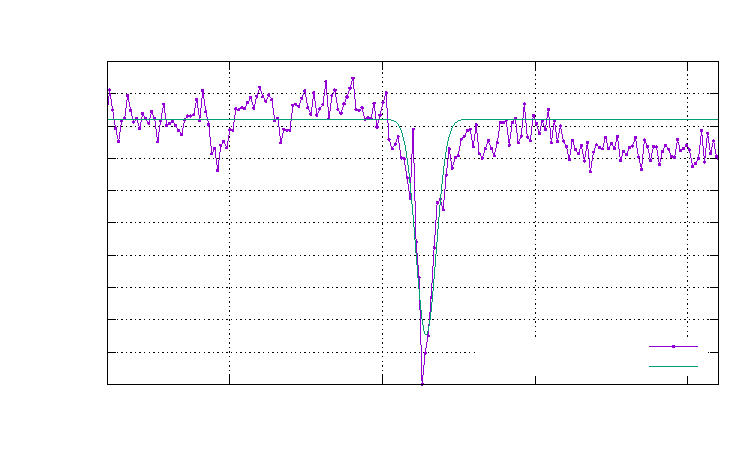
\includegraphics[width={360.00bp},height={216.00bp}]{134083-F5_gauss}}%
    \gplfronttext
  \end{picture}%
\endgroup
}
  \caption{} \label{fig:2b}
\end{figure}
\begin{figure}[h]
  \centering
  \resizebox{.5\textwidth}{!}{% GNUPLOT: LaTeX picture with Postscript
\begingroup
  \makeatletter
  \providecommand\color[2][]{%
    \GenericError{(gnuplot) \space\space\space\@spaces}{%
      Package color not loaded in conjunction with
      terminal option `colourtext'%
    }{See the gnuplot documentation for explanation.%
    }{Either use 'blacktext' in gnuplot or load the package
      color.sty in LaTeX.}%
    \renewcommand\color[2][]{}%
  }%
  \providecommand\includegraphics[2][]{%
    \GenericError{(gnuplot) \space\space\space\@spaces}{%
      Package graphicx or graphics not loaded%
    }{See the gnuplot documentation for explanation.%
    }{The gnuplot epslatex terminal needs graphicx.sty or graphics.sty.}%
    \renewcommand\includegraphics[2][]{}%
  }%
  \providecommand\rotatebox[2]{#2}%
  \@ifundefined{ifGPcolor}{%
    \newif\ifGPcolor
    \GPcolortrue
  }{}%
  \@ifundefined{ifGPblacktext}{%
    \newif\ifGPblacktext
    \GPblacktexttrue
  }{}%
  % define a \g@addto@macro without @ in the name:
  \let\gplgaddtomacro\g@addto@macro
  % define empty templates for all commands taking text:
  \gdef\gplbacktext{}%
  \gdef\gplfronttext{}%
  \makeatother
  \ifGPblacktext
    % no textcolor at all
    \def\colorrgb#1{}%
    \def\colorgray#1{}%
  \else
    % gray or color?
    \ifGPcolor
      \def\colorrgb#1{\color[rgb]{#1}}%
      \def\colorgray#1{\color[gray]{#1}}%
      \expandafter\def\csname LTw\endcsname{\color{white}}%
      \expandafter\def\csname LTb\endcsname{\color{black}}%
      \expandafter\def\csname LTa\endcsname{\color{black}}%
      \expandafter\def\csname LT0\endcsname{\color[rgb]{1,0,0}}%
      \expandafter\def\csname LT1\endcsname{\color[rgb]{0,1,0}}%
      \expandafter\def\csname LT2\endcsname{\color[rgb]{0,0,1}}%
      \expandafter\def\csname LT3\endcsname{\color[rgb]{1,0,1}}%
      \expandafter\def\csname LT4\endcsname{\color[rgb]{0,1,1}}%
      \expandafter\def\csname LT5\endcsname{\color[rgb]{1,1,0}}%
      \expandafter\def\csname LT6\endcsname{\color[rgb]{0,0,0}}%
      \expandafter\def\csname LT7\endcsname{\color[rgb]{1,0.3,0}}%
      \expandafter\def\csname LT8\endcsname{\color[rgb]{0.5,0.5,0.5}}%
    \else
      % gray
      \def\colorrgb#1{\color{black}}%
      \def\colorgray#1{\color[gray]{#1}}%
      \expandafter\def\csname LTw\endcsname{\color{white}}%
      \expandafter\def\csname LTb\endcsname{\color{black}}%
      \expandafter\def\csname LTa\endcsname{\color{black}}%
      \expandafter\def\csname LT0\endcsname{\color{black}}%
      \expandafter\def\csname LT1\endcsname{\color{black}}%
      \expandafter\def\csname LT2\endcsname{\color{black}}%
      \expandafter\def\csname LT3\endcsname{\color{black}}%
      \expandafter\def\csname LT4\endcsname{\color{black}}%
      \expandafter\def\csname LT5\endcsname{\color{black}}%
      \expandafter\def\csname LT6\endcsname{\color{black}}%
      \expandafter\def\csname LT7\endcsname{\color{black}}%
      \expandafter\def\csname LT8\endcsname{\color{black}}%
    \fi
  \fi
    \setlength{\unitlength}{0.0500bp}%
    \ifx\gptboxheight\undefined%
      \newlength{\gptboxheight}%
      \newlength{\gptboxwidth}%
      \newsavebox{\gptboxtext}%
    \fi%
    \setlength{\fboxrule}{0.5pt}%
    \setlength{\fboxsep}{1pt}%
    \definecolor{tbcol}{rgb}{1,1,1}%
\begin{picture}(7200.00,4320.00)%
    \gplgaddtomacro\gplbacktext{%
      \csname LTb\endcsname%%
      \put(1123,619){\makebox(0,0)[r]{\strut{}635\cdot10^{-9}}}%
      \csname LTb\endcsname%%
      \put(1123,963){\makebox(0,0)[r]{\strut{}640\cdot10^{-9}}}%
      \csname LTb\endcsname%%
      \put(1123,1308){\makebox(0,0)[r]{\strut{}645\cdot10^{-9}}}%
      \csname LTb\endcsname%%
      \put(1123,1652){\makebox(0,0)[r]{\strut{}650\cdot10^{-9}}}%
      \csname LTb\endcsname%%
      \put(1123,1997){\makebox(0,0)[r]{\strut{}655\cdot10^{-9}}}%
      \csname LTb\endcsname%%
      \put(1123,2341){\makebox(0,0)[r]{\strut{}660\cdot10^{-9}}}%
      \csname LTb\endcsname%%
      \put(1123,2686){\makebox(0,0)[r]{\strut{}665\cdot10^{-9}}}%
      \csname LTb\endcsname%%
      \put(1123,3030){\makebox(0,0)[r]{\strut{}670\cdot10^{-9}}}%
      \csname LTb\endcsname%%
      \put(1123,3374){\makebox(0,0)[r]{\strut{}675\cdot10^{-9}}}%
      \csname LTb\endcsname%%
      \put(1123,3719){\makebox(0,0)[r]{\strut{}680\cdot10^{-9}}}%
      \csname LTb\endcsname%%
      \put(1221,425){\makebox(0,0){\strut{}$200$}}%
      \csname LTb\endcsname%%
      \put(1850,425){\makebox(0,0){\strut{}$250$}}%
      \csname LTb\endcsname%%
      \put(2480,425){\makebox(0,0){\strut{}$300$}}%
      \csname LTb\endcsname%%
      \put(3109,425){\makebox(0,0){\strut{}$350$}}%
      \csname LTb\endcsname%%
      \put(3739,425){\makebox(0,0){\strut{}$400$}}%
      \csname LTb\endcsname%%
      \put(4368,425){\makebox(0,0){\strut{}$450$}}%
      \csname LTb\endcsname%%
      \put(4997,425){\makebox(0,0){\strut{}$500$}}%
      \csname LTb\endcsname%%
      \put(5627,425){\makebox(0,0){\strut{}$550$}}%
      \csname LTb\endcsname%%
      \put(6256,425){\makebox(0,0){\strut{}$600$}}%
      \csname LTb\endcsname%%
      \put(6886,425){\makebox(0,0){\strut{}$650$}}%
    }%
    \gplgaddtomacro\gplfronttext{%
      \csname LTb\endcsname%%
      \put(6123,3545){\makebox(0,0)[r]{\strut{}Datenpunkte}}%
      \csname LTb\endcsname%%
      \put(6123,3351){\makebox(0,0)[r]{\strut{}Anpassung $\lambda_\text{f}(x)$}}%
      \csname LTb\endcsname%%
      \put(170,2169){\rotatebox{-270.00}{\makebox(0,0){\strut{}Wellenlänge $\lambda/\SI{}{m}$}}}%
      \csname LTb\endcsname%%
      \put(4053,135){\makebox(0,0){\strut{}Pixelkoordinate$/\textrm{Pixel}$}}%
      \csname LTb\endcsname%%
      \put(4053,4009){\makebox(0,0){\strut{}Kalibraiton des 134083-F5 Spektrums mit $\chi^2/\textrm{ddof}=\SI{1.45E-02}{}$}}%
    }%
    \gplbacktext
    \put(0,0){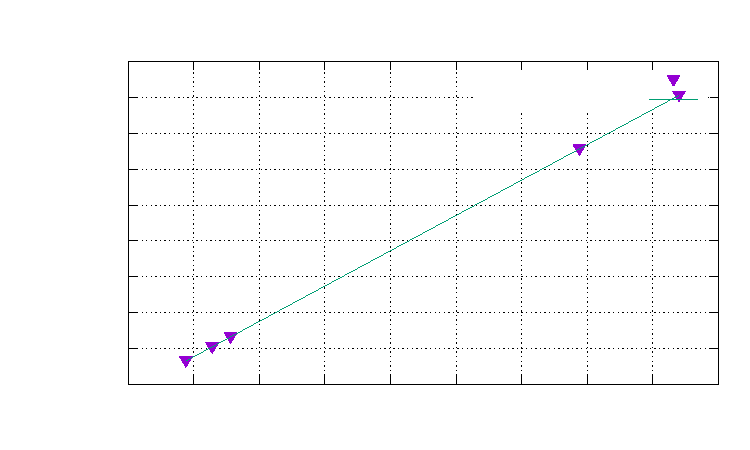
\includegraphics[width={360.00bp},height={216.00bp}]{134083-F5_kali}}%
    \gplfronttext
  \end{picture}%
\endgroup
}
  \caption{} \label{fig:2c}
\end{figure}
\begin{figure}[h]
  \centering
  \resizebox{.5\textwidth}{!}{% GNUPLOT: LaTeX picture with Postscript
\begingroup
  \makeatletter
  \providecommand\color[2][]{%
    \GenericError{(gnuplot) \space\space\space\@spaces}{%
      Package color not loaded in conjunction with
      terminal option `colourtext'%
    }{See the gnuplot documentation for explanation.%
    }{Either use 'blacktext' in gnuplot or load the package
      color.sty in LaTeX.}%
    \renewcommand\color[2][]{}%
  }%
  \providecommand\includegraphics[2][]{%
    \GenericError{(gnuplot) \space\space\space\@spaces}{%
      Package graphicx or graphics not loaded%
    }{See the gnuplot documentation for explanation.%
    }{The gnuplot epslatex terminal needs graphicx.sty or graphics.sty.}%
    \renewcommand\includegraphics[2][]{}%
  }%
  \providecommand\rotatebox[2]{#2}%
  \@ifundefined{ifGPcolor}{%
    \newif\ifGPcolor
    \GPcolortrue
  }{}%
  \@ifundefined{ifGPblacktext}{%
    \newif\ifGPblacktext
    \GPblacktexttrue
  }{}%
  % define a \g@addto@macro without @ in the name:
  \let\gplgaddtomacro\g@addto@macro
  % define empty templates for all commands taking text:
  \gdef\gplbacktext{}%
  \gdef\gplfronttext{}%
  \makeatother
  \ifGPblacktext
    % no textcolor at all
    \def\colorrgb#1{}%
    \def\colorgray#1{}%
  \else
    % gray or color?
    \ifGPcolor
      \def\colorrgb#1{\color[rgb]{#1}}%
      \def\colorgray#1{\color[gray]{#1}}%
      \expandafter\def\csname LTw\endcsname{\color{white}}%
      \expandafter\def\csname LTb\endcsname{\color{black}}%
      \expandafter\def\csname LTa\endcsname{\color{black}}%
      \expandafter\def\csname LT0\endcsname{\color[rgb]{1,0,0}}%
      \expandafter\def\csname LT1\endcsname{\color[rgb]{0,1,0}}%
      \expandafter\def\csname LT2\endcsname{\color[rgb]{0,0,1}}%
      \expandafter\def\csname LT3\endcsname{\color[rgb]{1,0,1}}%
      \expandafter\def\csname LT4\endcsname{\color[rgb]{0,1,1}}%
      \expandafter\def\csname LT5\endcsname{\color[rgb]{1,1,0}}%
      \expandafter\def\csname LT6\endcsname{\color[rgb]{0,0,0}}%
      \expandafter\def\csname LT7\endcsname{\color[rgb]{1,0.3,0}}%
      \expandafter\def\csname LT8\endcsname{\color[rgb]{0.5,0.5,0.5}}%
    \else
      % gray
      \def\colorrgb#1{\color{black}}%
      \def\colorgray#1{\color[gray]{#1}}%
      \expandafter\def\csname LTw\endcsname{\color{white}}%
      \expandafter\def\csname LTb\endcsname{\color{black}}%
      \expandafter\def\csname LTa\endcsname{\color{black}}%
      \expandafter\def\csname LT0\endcsname{\color{black}}%
      \expandafter\def\csname LT1\endcsname{\color{black}}%
      \expandafter\def\csname LT2\endcsname{\color{black}}%
      \expandafter\def\csname LT3\endcsname{\color{black}}%
      \expandafter\def\csname LT4\endcsname{\color{black}}%
      \expandafter\def\csname LT5\endcsname{\color{black}}%
      \expandafter\def\csname LT6\endcsname{\color{black}}%
      \expandafter\def\csname LT7\endcsname{\color{black}}%
      \expandafter\def\csname LT8\endcsname{\color{black}}%
    \fi
  \fi
    \setlength{\unitlength}{0.0500bp}%
    \ifx\gptboxheight\undefined%
      \newlength{\gptboxheight}%
      \newlength{\gptboxwidth}%
      \newsavebox{\gptboxtext}%
    \fi%
    \setlength{\fboxrule}{0.5pt}%
    \setlength{\fboxsep}{1pt}%
    \definecolor{tbcol}{rgb}{1,1,1}%
\begin{picture}(7200.00,4320.00)%
    \gplgaddtomacro\gplbacktext{%
      \csname LTb\endcsname%%
      \put(1123,619){\makebox(0,0)[r]{\strut{}$400\cdot10^{-3}$}}%
      \csname LTb\endcsname%%
      \put(1123,1135){\makebox(0,0)[r]{\strut{}$500\cdot10^{-3}$}}%
      \csname LTb\endcsname%%
      \put(1123,1652){\makebox(0,0)[r]{\strut{}$600\cdot10^{-3}$}}%
      \csname LTb\endcsname%%
      \put(1123,2169){\makebox(0,0)[r]{\strut{}$700\cdot10^{-3}$}}%
      \csname LTb\endcsname%%
      \put(1123,2686){\makebox(0,0)[r]{\strut{}$800\cdot10^{-3}$}}%
      \csname LTb\endcsname%%
      \put(1123,3202){\makebox(0,0)[r]{\strut{}$900\cdot10^{-3}$}}%
      \csname LTb\endcsname%%
      \put(1123,3719){\makebox(0,0)[r]{\strut{}$1\cdot10^{0}$}}%
      \csname LTb\endcsname%%
      \put(1221,425){\makebox(0,0){\strut{}$0$}}%
      \csname LTb\endcsname%%
      \put(1929,425){\makebox(0,0){\strut{}$100$}}%
      \csname LTb\endcsname%%
      \put(2637,425){\makebox(0,0){\strut{}$200$}}%
      \csname LTb\endcsname%%
      \put(3345,425){\makebox(0,0){\strut{}$300$}}%
      \csname LTb\endcsname%%
      \put(4053,425){\makebox(0,0){\strut{}$400$}}%
      \csname LTb\endcsname%%
      \put(4761,425){\makebox(0,0){\strut{}$500$}}%
      \csname LTb\endcsname%%
      \put(5470,425){\makebox(0,0){\strut{}$600$}}%
      \csname LTb\endcsname%%
      \put(6178,425){\makebox(0,0){\strut{}$700$}}%
      \csname LTb\endcsname%%
      \put(6886,425){\makebox(0,0){\strut{}$800$}}%
    }%
    \gplgaddtomacro\gplfronttext{%
      \csname LTb\endcsname%%
      \put(170,2169){\rotatebox{-270}{\makebox(0,0){\strut{}Amplitude$/\textrm{a.u.}$}}}%
      \csname LTb\endcsname%%
      \put(4053,135){\makebox(0,0){\strut{}Pixelkoordinate$/\textrm{Pixel}$}}%
      \csname LTb\endcsname%%
      \put(6123,3545){\makebox(0,0)[r]{\strut{}21428-B3}}%
      \csname LTb\endcsname%%
      \put(6123,3351){\makebox(0,0)[r]{\strut{}Kalibrationslampe}}%
      \csname LTb\endcsname%%
      \put(4053,4009){\makebox(0,0){\strut{}Spektrum}}%
    }%
    \gplbacktext
    \put(0,0){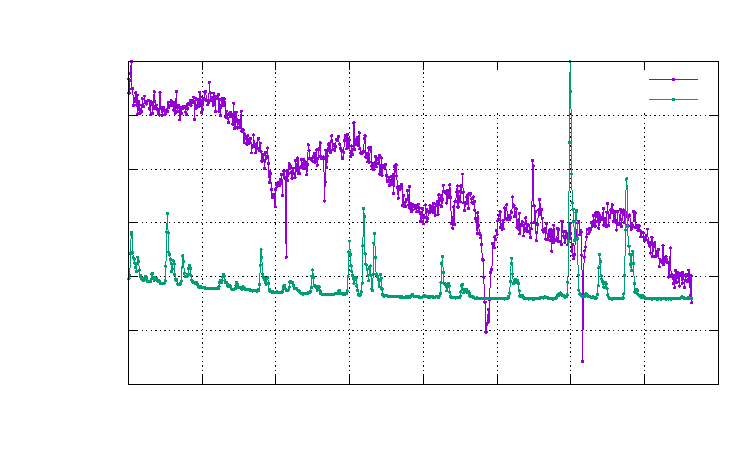
\includegraphics[width={360.00bp},height={216.00bp}]{21428-B3_data}}%
    \gplfronttext
  \end{picture}%
\endgroup
}
  \caption{} \label{fig:3a}
\end{figure} 
\begin{figure}[h]
  \centering
  \resizebox{.5\textwidth}{!}{% GNUPLOT: LaTeX picture with Postscript
\begingroup
  \makeatletter
  \providecommand\color[2][]{%
    \GenericError{(gnuplot) \space\space\space\@spaces}{%
      Package color not loaded in conjunction with
      terminal option `colourtext'%
    }{See the gnuplot documentation for explanation.%
    }{Either use 'blacktext' in gnuplot or load the package
      color.sty in LaTeX.}%
    \renewcommand\color[2][]{}%
  }%
  \providecommand\includegraphics[2][]{%
    \GenericError{(gnuplot) \space\space\space\@spaces}{%
      Package graphicx or graphics not loaded%
    }{See the gnuplot documentation for explanation.%
    }{The gnuplot epslatex terminal needs graphicx.sty or graphics.sty.}%
    \renewcommand\includegraphics[2][]{}%
  }%
  \providecommand\rotatebox[2]{#2}%
  \@ifundefined{ifGPcolor}{%
    \newif\ifGPcolor
    \GPcolortrue
  }{}%
  \@ifundefined{ifGPblacktext}{%
    \newif\ifGPblacktext
    \GPblacktexttrue
  }{}%
  % define a \g@addto@macro without @ in the name:
  \let\gplgaddtomacro\g@addto@macro
  % define empty templates for all commands taking text:
  \gdef\gplbacktext{}%
  \gdef\gplfronttext{}%
  \makeatother
  \ifGPblacktext
    % no textcolor at all
    \def\colorrgb#1{}%
    \def\colorgray#1{}%
  \else
    % gray or color?
    \ifGPcolor
      \def\colorrgb#1{\color[rgb]{#1}}%
      \def\colorgray#1{\color[gray]{#1}}%
      \expandafter\def\csname LTw\endcsname{\color{white}}%
      \expandafter\def\csname LTb\endcsname{\color{black}}%
      \expandafter\def\csname LTa\endcsname{\color{black}}%
      \expandafter\def\csname LT0\endcsname{\color[rgb]{1,0,0}}%
      \expandafter\def\csname LT1\endcsname{\color[rgb]{0,1,0}}%
      \expandafter\def\csname LT2\endcsname{\color[rgb]{0,0,1}}%
      \expandafter\def\csname LT3\endcsname{\color[rgb]{1,0,1}}%
      \expandafter\def\csname LT4\endcsname{\color[rgb]{0,1,1}}%
      \expandafter\def\csname LT5\endcsname{\color[rgb]{1,1,0}}%
      \expandafter\def\csname LT6\endcsname{\color[rgb]{0,0,0}}%
      \expandafter\def\csname LT7\endcsname{\color[rgb]{1,0.3,0}}%
      \expandafter\def\csname LT8\endcsname{\color[rgb]{0.5,0.5,0.5}}%
    \else
      % gray
      \def\colorrgb#1{\color{black}}%
      \def\colorgray#1{\color[gray]{#1}}%
      \expandafter\def\csname LTw\endcsname{\color{white}}%
      \expandafter\def\csname LTb\endcsname{\color{black}}%
      \expandafter\def\csname LTa\endcsname{\color{black}}%
      \expandafter\def\csname LT0\endcsname{\color{black}}%
      \expandafter\def\csname LT1\endcsname{\color{black}}%
      \expandafter\def\csname LT2\endcsname{\color{black}}%
      \expandafter\def\csname LT3\endcsname{\color{black}}%
      \expandafter\def\csname LT4\endcsname{\color{black}}%
      \expandafter\def\csname LT5\endcsname{\color{black}}%
      \expandafter\def\csname LT6\endcsname{\color{black}}%
      \expandafter\def\csname LT7\endcsname{\color{black}}%
      \expandafter\def\csname LT8\endcsname{\color{black}}%
    \fi
  \fi
    \setlength{\unitlength}{0.0500bp}%
    \ifx\gptboxheight\undefined%
      \newlength{\gptboxheight}%
      \newlength{\gptboxwidth}%
      \newsavebox{\gptboxtext}%
    \fi%
    \setlength{\fboxrule}{0.5pt}%
    \setlength{\fboxsep}{1pt}%
    \definecolor{tbcol}{rgb}{1,1,1}%
\begin{picture}(7200.00,4320.00)%
    \gplgaddtomacro\gplbacktext{%
      \csname LTb\endcsname%%
      \put(927,619){\makebox(0,0)[r]{\strut{}15\cdot10^{3}}}%
      \csname LTb\endcsname%%
      \put(927,901){\makebox(0,0)[r]{\strut{}16\cdot10^{3}}}%
      \csname LTb\endcsname%%
      \put(927,1182){\makebox(0,0)[r]{\strut{}17\cdot10^{3}}}%
      \csname LTb\endcsname%%
      \put(927,1464){\makebox(0,0)[r]{\strut{}18\cdot10^{3}}}%
      \csname LTb\endcsname%%
      \put(927,1746){\makebox(0,0)[r]{\strut{}19\cdot10^{3}}}%
      \csname LTb\endcsname%%
      \put(927,2028){\makebox(0,0)[r]{\strut{}20\cdot10^{3}}}%
      \csname LTb\endcsname%%
      \put(927,2310){\makebox(0,0)[r]{\strut{}21\cdot10^{3}}}%
      \csname LTb\endcsname%%
      \put(927,2592){\makebox(0,0)[r]{\strut{}22\cdot10^{3}}}%
      \csname LTb\endcsname%%
      \put(927,2873){\makebox(0,0)[r]{\strut{}23\cdot10^{3}}}%
      \csname LTb\endcsname%%
      \put(927,3155){\makebox(0,0)[r]{\strut{}24\cdot10^{3}}}%
      \csname LTb\endcsname%%
      \put(927,3437){\makebox(0,0)[r]{\strut{}25\cdot10^{3}}}%
      \csname LTb\endcsname%%
      \put(927,3719){\makebox(0,0)[r]{\strut{}26\cdot10^{3}}}%
      \csname LTb\endcsname%%
      \put(2197,425){\makebox(0,0){\strut{}650\cdot10^{-9}}}%
      \csname LTb\endcsname%%
      \put(3662,425){\makebox(0,0){\strut{}655\cdot10^{-9}}}%
      \csname LTb\endcsname%%
      \put(5128,425){\makebox(0,0){\strut{}660\cdot10^{-9}}}%
      \csname LTb\endcsname%%
      \put(6593,425){\makebox(0,0){\strut{}665\cdot10^{-9}}}%
    }%
    \gplgaddtomacro\gplfronttext{%
      \csname LTb\endcsname%%
      \put(6123,986){\makebox(0,0)[r]{\strut{}Datenpunkte}}%
      \csname LTb\endcsname%%
      \put(6123,793){\makebox(0,0)[r]{\strut{}Anpassung $G_\text{f}(x)$}}%
      \csname LTb\endcsname%%
      \put(170,2169){\rotatebox{-270.00}{\makebox(0,0){\strut{}Amplitude$/\textrm{a.u.}$}}}%
      \csname LTb\endcsname%%
      \put(3955,135){\makebox(0,0){\strut{}Wellenlänge $\lambda/\SI{}{m}$}}%
      \csname LTb\endcsname%%
      \put(3955,4009){\makebox(0,0){\strut{}H$\alpha$(\SI{656}{nm})-Linie von 21428-B3 mit $\chi^2/\textrm{ddof}=\SI{4.66E-01}{}$}}%
    }%
    \gplbacktext
    \put(0,0){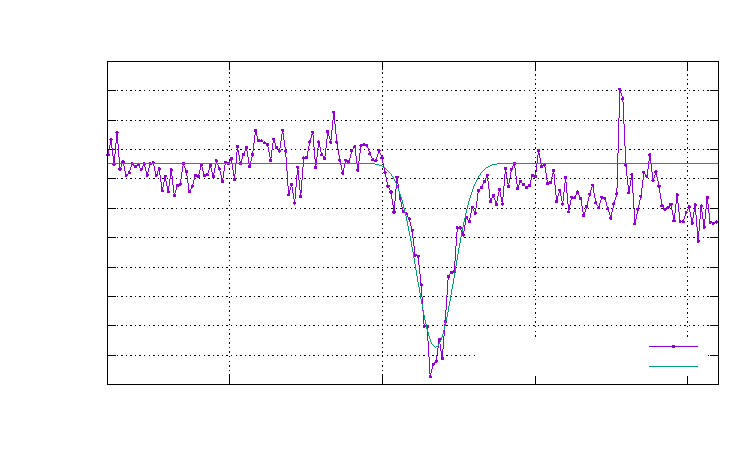
\includegraphics[width={360.00bp},height={216.00bp}]{21428-B3_gauss}}%
    \gplfronttext
  \end{picture}%
\endgroup
}
  \caption{} \label{fig:3b}
\end{figure}
\begin{figure}[h]
  \centering
  \resizebox{.5\textwidth}{!}{% GNUPLOT: LaTeX picture with Postscript
\begingroup
  \makeatletter
  \providecommand\color[2][]{%
    \GenericError{(gnuplot) \space\space\space\@spaces}{%
      Package color not loaded in conjunction with
      terminal option `colourtext'%
    }{See the gnuplot documentation for explanation.%
    }{Either use 'blacktext' in gnuplot or load the package
      color.sty in LaTeX.}%
    \renewcommand\color[2][]{}%
  }%
  \providecommand\includegraphics[2][]{%
    \GenericError{(gnuplot) \space\space\space\@spaces}{%
      Package graphicx or graphics not loaded%
    }{See the gnuplot documentation for explanation.%
    }{The gnuplot epslatex terminal needs graphicx.sty or graphics.sty.}%
    \renewcommand\includegraphics[2][]{}%
  }%
  \providecommand\rotatebox[2]{#2}%
  \@ifundefined{ifGPcolor}{%
    \newif\ifGPcolor
    \GPcolortrue
  }{}%
  \@ifundefined{ifGPblacktext}{%
    \newif\ifGPblacktext
    \GPblacktexttrue
  }{}%
  % define a \g@addto@macro without @ in the name:
  \let\gplgaddtomacro\g@addto@macro
  % define empty templates for all commands taking text:
  \gdef\gplbacktext{}%
  \gdef\gplfronttext{}%
  \makeatother
  \ifGPblacktext
    % no textcolor at all
    \def\colorrgb#1{}%
    \def\colorgray#1{}%
  \else
    % gray or color?
    \ifGPcolor
      \def\colorrgb#1{\color[rgb]{#1}}%
      \def\colorgray#1{\color[gray]{#1}}%
      \expandafter\def\csname LTw\endcsname{\color{white}}%
      \expandafter\def\csname LTb\endcsname{\color{black}}%
      \expandafter\def\csname LTa\endcsname{\color{black}}%
      \expandafter\def\csname LT0\endcsname{\color[rgb]{1,0,0}}%
      \expandafter\def\csname LT1\endcsname{\color[rgb]{0,1,0}}%
      \expandafter\def\csname LT2\endcsname{\color[rgb]{0,0,1}}%
      \expandafter\def\csname LT3\endcsname{\color[rgb]{1,0,1}}%
      \expandafter\def\csname LT4\endcsname{\color[rgb]{0,1,1}}%
      \expandafter\def\csname LT5\endcsname{\color[rgb]{1,1,0}}%
      \expandafter\def\csname LT6\endcsname{\color[rgb]{0,0,0}}%
      \expandafter\def\csname LT7\endcsname{\color[rgb]{1,0.3,0}}%
      \expandafter\def\csname LT8\endcsname{\color[rgb]{0.5,0.5,0.5}}%
    \else
      % gray
      \def\colorrgb#1{\color{black}}%
      \def\colorgray#1{\color[gray]{#1}}%
      \expandafter\def\csname LTw\endcsname{\color{white}}%
      \expandafter\def\csname LTb\endcsname{\color{black}}%
      \expandafter\def\csname LTa\endcsname{\color{black}}%
      \expandafter\def\csname LT0\endcsname{\color{black}}%
      \expandafter\def\csname LT1\endcsname{\color{black}}%
      \expandafter\def\csname LT2\endcsname{\color{black}}%
      \expandafter\def\csname LT3\endcsname{\color{black}}%
      \expandafter\def\csname LT4\endcsname{\color{black}}%
      \expandafter\def\csname LT5\endcsname{\color{black}}%
      \expandafter\def\csname LT6\endcsname{\color{black}}%
      \expandafter\def\csname LT7\endcsname{\color{black}}%
      \expandafter\def\csname LT8\endcsname{\color{black}}%
    \fi
  \fi
    \setlength{\unitlength}{0.0500bp}%
    \ifx\gptboxheight\undefined%
      \newlength{\gptboxheight}%
      \newlength{\gptboxwidth}%
      \newsavebox{\gptboxtext}%
    \fi%
    \setlength{\fboxrule}{0.5pt}%
    \setlength{\fboxsep}{1pt}%
    \definecolor{tbcol}{rgb}{1,1,1}%
\begin{picture}(7200.00,4320.00)%
    \gplgaddtomacro\gplbacktext{%
      \csname LTb\endcsname%%
      \put(1123,619){\makebox(0,0)[r]{\strut{}$635\cdot10^{-9}$}}%
      \csname LTb\endcsname%%
      \put(1123,963){\makebox(0,0)[r]{\strut{}$640\cdot10^{-9}$}}%
      \csname LTb\endcsname%%
      \put(1123,1308){\makebox(0,0)[r]{\strut{}$645\cdot10^{-9}$}}%
      \csname LTb\endcsname%%
      \put(1123,1652){\makebox(0,0)[r]{\strut{}$650\cdot10^{-9}$}}%
      \csname LTb\endcsname%%
      \put(1123,1997){\makebox(0,0)[r]{\strut{}$655\cdot10^{-9}$}}%
      \csname LTb\endcsname%%
      \put(1123,2341){\makebox(0,0)[r]{\strut{}$660\cdot10^{-9}$}}%
      \csname LTb\endcsname%%
      \put(1123,2686){\makebox(0,0)[r]{\strut{}$665\cdot10^{-9}$}}%
      \csname LTb\endcsname%%
      \put(1123,3030){\makebox(0,0)[r]{\strut{}$670\cdot10^{-9}$}}%
      \csname LTb\endcsname%%
      \put(1123,3374){\makebox(0,0)[r]{\strut{}$675\cdot10^{-9}$}}%
      \csname LTb\endcsname%%
      \put(1123,3719){\makebox(0,0)[r]{\strut{}$680\cdot10^{-9}$}}%
      \csname LTb\endcsname%%
      \put(1221,425){\makebox(0,0){\strut{}$300$}}%
      \csname LTb\endcsname%%
      \put(1929,425){\makebox(0,0){\strut{}$350$}}%
      \csname LTb\endcsname%%
      \put(2637,425){\makebox(0,0){\strut{}$400$}}%
      \csname LTb\endcsname%%
      \put(3345,425){\makebox(0,0){\strut{}$450$}}%
      \csname LTb\endcsname%%
      \put(4053,425){\makebox(0,0){\strut{}$500$}}%
      \csname LTb\endcsname%%
      \put(4761,425){\makebox(0,0){\strut{}$550$}}%
      \csname LTb\endcsname%%
      \put(5470,425){\makebox(0,0){\strut{}$600$}}%
      \csname LTb\endcsname%%
      \put(6178,425){\makebox(0,0){\strut{}$650$}}%
      \csname LTb\endcsname%%
      \put(6886,425){\makebox(0,0){\strut{}$700$}}%
    }%
    \gplgaddtomacro\gplfronttext{%
      \csname LTb\endcsname%%
      \put(170,2169){\rotatebox{-270}{\makebox(0,0){\strut{}Wellenlänge $\lambda/\SI{}{m}$}}}%
      \csname LTb\endcsname%%
      \put(4053,135){\makebox(0,0){\strut{}Pixelkoordinate$/\textrm{Pixel}$}}%
      \csname LTb\endcsname%%
      \put(6123,3545){\makebox(0,0)[r]{\strut{}Datenpunkte}}%
      \csname LTb\endcsname%%
      \put(6123,3351){\makebox(0,0)[r]{\strut{}Anpassung $\lambda_\text{f}(x)$}}%
      \csname LTb\endcsname%%
      \put(4053,4009){\makebox(0,0){\strut{}Kalibraiton des 21428-B3 Spektrums mit $\chi^2/\textrm{ddof}=\SI{3.03E-02}{}$}}%
    }%
    \gplbacktext
    \put(0,0){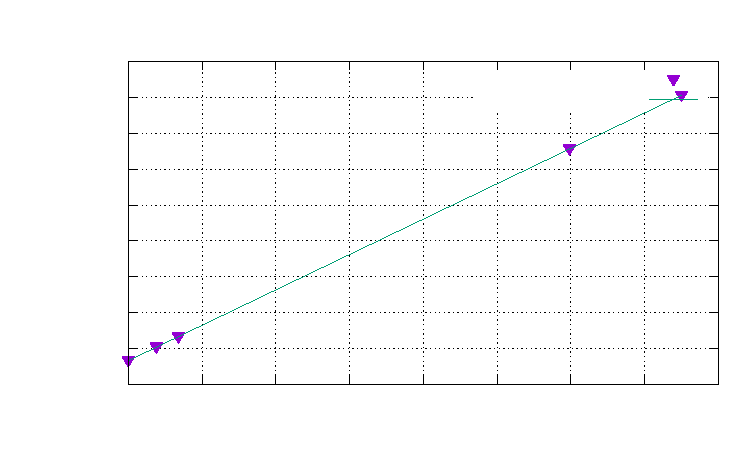
\includegraphics[width={360.00bp},height={216.00bp}]{21428-B3_kali}}%
    \gplfronttext
  \end{picture}%
\endgroup
}
  \caption{} \label{fig:3c}
\end{figure}
\begin{figure}[h]
  \centering
  \resizebox{.5\textwidth}{!}{% GNUPLOT: LaTeX picture with Postscript
\begingroup
  \makeatletter
  \providecommand\color[2][]{%
    \GenericError{(gnuplot) \space\space\space\@spaces}{%
      Package color not loaded in conjunction with
      terminal option `colourtext'%
    }{See the gnuplot documentation for explanation.%
    }{Either use 'blacktext' in gnuplot or load the package
      color.sty in LaTeX.}%
    \renewcommand\color[2][]{}%
  }%
  \providecommand\includegraphics[2][]{%
    \GenericError{(gnuplot) \space\space\space\@spaces}{%
      Package graphicx or graphics not loaded%
    }{See the gnuplot documentation for explanation.%
    }{The gnuplot epslatex terminal needs graphicx.sty or graphics.sty.}%
    \renewcommand\includegraphics[2][]{}%
  }%
  \providecommand\rotatebox[2]{#2}%
  \@ifundefined{ifGPcolor}{%
    \newif\ifGPcolor
    \GPcolortrue
  }{}%
  \@ifundefined{ifGPblacktext}{%
    \newif\ifGPblacktext
    \GPblacktexttrue
  }{}%
  % define a \g@addto@macro without @ in the name:
  \let\gplgaddtomacro\g@addto@macro
  % define empty templates for all commands taking text:
  \gdef\gplbacktext{}%
  \gdef\gplfronttext{}%
  \makeatother
  \ifGPblacktext
    % no textcolor at all
    \def\colorrgb#1{}%
    \def\colorgray#1{}%
  \else
    % gray or color?
    \ifGPcolor
      \def\colorrgb#1{\color[rgb]{#1}}%
      \def\colorgray#1{\color[gray]{#1}}%
      \expandafter\def\csname LTw\endcsname{\color{white}}%
      \expandafter\def\csname LTb\endcsname{\color{black}}%
      \expandafter\def\csname LTa\endcsname{\color{black}}%
      \expandafter\def\csname LT0\endcsname{\color[rgb]{1,0,0}}%
      \expandafter\def\csname LT1\endcsname{\color[rgb]{0,1,0}}%
      \expandafter\def\csname LT2\endcsname{\color[rgb]{0,0,1}}%
      \expandafter\def\csname LT3\endcsname{\color[rgb]{1,0,1}}%
      \expandafter\def\csname LT4\endcsname{\color[rgb]{0,1,1}}%
      \expandafter\def\csname LT5\endcsname{\color[rgb]{1,1,0}}%
      \expandafter\def\csname LT6\endcsname{\color[rgb]{0,0,0}}%
      \expandafter\def\csname LT7\endcsname{\color[rgb]{1,0.3,0}}%
      \expandafter\def\csname LT8\endcsname{\color[rgb]{0.5,0.5,0.5}}%
    \else
      % gray
      \def\colorrgb#1{\color{black}}%
      \def\colorgray#1{\color[gray]{#1}}%
      \expandafter\def\csname LTw\endcsname{\color{white}}%
      \expandafter\def\csname LTb\endcsname{\color{black}}%
      \expandafter\def\csname LTa\endcsname{\color{black}}%
      \expandafter\def\csname LT0\endcsname{\color{black}}%
      \expandafter\def\csname LT1\endcsname{\color{black}}%
      \expandafter\def\csname LT2\endcsname{\color{black}}%
      \expandafter\def\csname LT3\endcsname{\color{black}}%
      \expandafter\def\csname LT4\endcsname{\color{black}}%
      \expandafter\def\csname LT5\endcsname{\color{black}}%
      \expandafter\def\csname LT6\endcsname{\color{black}}%
      \expandafter\def\csname LT7\endcsname{\color{black}}%
      \expandafter\def\csname LT8\endcsname{\color{black}}%
    \fi
  \fi
    \setlength{\unitlength}{0.0500bp}%
    \ifx\gptboxheight\undefined%
      \newlength{\gptboxheight}%
      \newlength{\gptboxwidth}%
      \newsavebox{\gptboxtext}%
    \fi%
    \setlength{\fboxrule}{0.5pt}%
    \setlength{\fboxsep}{1pt}%
    \definecolor{tbcol}{rgb}{1,1,1}%
\begin{picture}(7200.00,4320.00)%
    \gplgaddtomacro\gplbacktext{%
      \csname LTb\endcsname%%
      \put(1123,619){\makebox(0,0)[r]{\strut{}$300\cdot10^{-3}$}}%
      \csname LTb\endcsname%%
      \put(1123,1062){\makebox(0,0)[r]{\strut{}$400\cdot10^{-3}$}}%
      \csname LTb\endcsname%%
      \put(1123,1505){\makebox(0,0)[r]{\strut{}$500\cdot10^{-3}$}}%
      \csname LTb\endcsname%%
      \put(1123,1947){\makebox(0,0)[r]{\strut{}$600\cdot10^{-3}$}}%
      \csname LTb\endcsname%%
      \put(1123,2390){\makebox(0,0)[r]{\strut{}$700\cdot10^{-3}$}}%
      \csname LTb\endcsname%%
      \put(1123,2833){\makebox(0,0)[r]{\strut{}$800\cdot10^{-3}$}}%
      \csname LTb\endcsname%%
      \put(1123,3276){\makebox(0,0)[r]{\strut{}$900\cdot10^{-3}$}}%
      \csname LTb\endcsname%%
      \put(1123,3719){\makebox(0,0)[r]{\strut{}$1\cdot10^{0}$}}%
      \csname LTb\endcsname%%
      \put(1221,425){\makebox(0,0){\strut{}$0$}}%
      \csname LTb\endcsname%%
      \put(1929,425){\makebox(0,0){\strut{}$100$}}%
      \csname LTb\endcsname%%
      \put(2637,425){\makebox(0,0){\strut{}$200$}}%
      \csname LTb\endcsname%%
      \put(3345,425){\makebox(0,0){\strut{}$300$}}%
      \csname LTb\endcsname%%
      \put(4053,425){\makebox(0,0){\strut{}$400$}}%
      \csname LTb\endcsname%%
      \put(4761,425){\makebox(0,0){\strut{}$500$}}%
      \csname LTb\endcsname%%
      \put(5470,425){\makebox(0,0){\strut{}$600$}}%
      \csname LTb\endcsname%%
      \put(6178,425){\makebox(0,0){\strut{}$700$}}%
      \csname LTb\endcsname%%
      \put(6886,425){\makebox(0,0){\strut{}$800$}}%
    }%
    \gplgaddtomacro\gplfronttext{%
      \csname LTb\endcsname%%
      \put(170,2169){\rotatebox{-270}{\makebox(0,0){\strut{}Amplitude$/\textrm{a.u.}$}}}%
      \csname LTb\endcsname%%
      \put(4053,135){\makebox(0,0){\strut{}Pixelkoordinate$/\textrm{Pixel}$}}%
      \csname LTb\endcsname%%
      \put(6123,3545){\makebox(0,0)[r]{\strut{}29488-A5}}%
      \csname LTb\endcsname%%
      \put(6123,3351){\makebox(0,0)[r]{\strut{}Kalibrationslampe}}%
      \csname LTb\endcsname%%
      \put(4053,4009){\makebox(0,0){\strut{}Spektrum}}%
    }%
    \gplbacktext
    \put(0,0){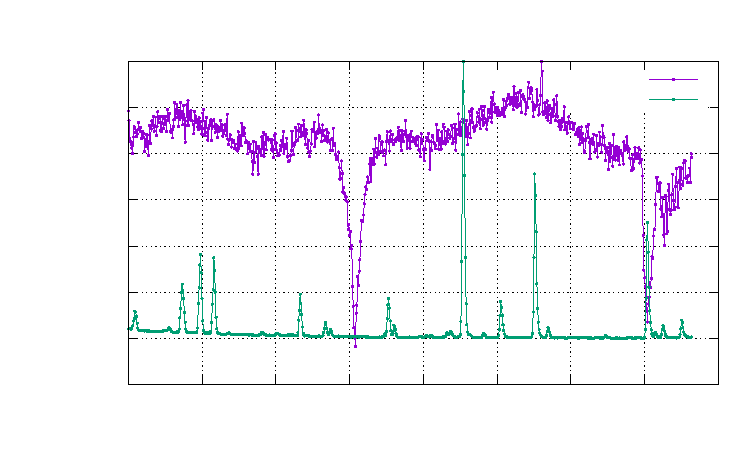
\includegraphics[width={360.00bp},height={216.00bp}]{29488-A5_data}}%
    \gplfronttext
  \end{picture}%
\endgroup
}
  \caption{} \label{fig:4a}
\end{figure}
\begin{figure}[h]
  \centering
  \resizebox{.5\textwidth}{!}{% GNUPLOT: LaTeX picture with Postscript
\begingroup
  \makeatletter
  \providecommand\color[2][]{%
    \GenericError{(gnuplot) \space\space\space\@spaces}{%
      Package color not loaded in conjunction with
      terminal option `colourtext'%
    }{See the gnuplot documentation for explanation.%
    }{Either use 'blacktext' in gnuplot or load the package
      color.sty in LaTeX.}%
    \renewcommand\color[2][]{}%
  }%
  \providecommand\includegraphics[2][]{%
    \GenericError{(gnuplot) \space\space\space\@spaces}{%
      Package graphicx or graphics not loaded%
    }{See the gnuplot documentation for explanation.%
    }{The gnuplot epslatex terminal needs graphicx.sty or graphics.sty.}%
    \renewcommand\includegraphics[2][]{}%
  }%
  \providecommand\rotatebox[2]{#2}%
  \@ifundefined{ifGPcolor}{%
    \newif\ifGPcolor
    \GPcolortrue
  }{}%
  \@ifundefined{ifGPblacktext}{%
    \newif\ifGPblacktext
    \GPblacktexttrue
  }{}%
  % define a \g@addto@macro without @ in the name:
  \let\gplgaddtomacro\g@addto@macro
  % define empty templates for all commands taking text:
  \gdef\gplbacktext{}%
  \gdef\gplfronttext{}%
  \makeatother
  \ifGPblacktext
    % no textcolor at all
    \def\colorrgb#1{}%
    \def\colorgray#1{}%
  \else
    % gray or color?
    \ifGPcolor
      \def\colorrgb#1{\color[rgb]{#1}}%
      \def\colorgray#1{\color[gray]{#1}}%
      \expandafter\def\csname LTw\endcsname{\color{white}}%
      \expandafter\def\csname LTb\endcsname{\color{black}}%
      \expandafter\def\csname LTa\endcsname{\color{black}}%
      \expandafter\def\csname LT0\endcsname{\color[rgb]{1,0,0}}%
      \expandafter\def\csname LT1\endcsname{\color[rgb]{0,1,0}}%
      \expandafter\def\csname LT2\endcsname{\color[rgb]{0,0,1}}%
      \expandafter\def\csname LT3\endcsname{\color[rgb]{1,0,1}}%
      \expandafter\def\csname LT4\endcsname{\color[rgb]{0,1,1}}%
      \expandafter\def\csname LT5\endcsname{\color[rgb]{1,1,0}}%
      \expandafter\def\csname LT6\endcsname{\color[rgb]{0,0,0}}%
      \expandafter\def\csname LT7\endcsname{\color[rgb]{1,0.3,0}}%
      \expandafter\def\csname LT8\endcsname{\color[rgb]{0.5,0.5,0.5}}%
    \else
      % gray
      \def\colorrgb#1{\color{black}}%
      \def\colorgray#1{\color[gray]{#1}}%
      \expandafter\def\csname LTw\endcsname{\color{white}}%
      \expandafter\def\csname LTb\endcsname{\color{black}}%
      \expandafter\def\csname LTa\endcsname{\color{black}}%
      \expandafter\def\csname LT0\endcsname{\color{black}}%
      \expandafter\def\csname LT1\endcsname{\color{black}}%
      \expandafter\def\csname LT2\endcsname{\color{black}}%
      \expandafter\def\csname LT3\endcsname{\color{black}}%
      \expandafter\def\csname LT4\endcsname{\color{black}}%
      \expandafter\def\csname LT5\endcsname{\color{black}}%
      \expandafter\def\csname LT6\endcsname{\color{black}}%
      \expandafter\def\csname LT7\endcsname{\color{black}}%
      \expandafter\def\csname LT8\endcsname{\color{black}}%
    \fi
  \fi
    \setlength{\unitlength}{0.0500bp}%
    \ifx\gptboxheight\undefined%
      \newlength{\gptboxheight}%
      \newlength{\gptboxwidth}%
      \newsavebox{\gptboxtext}%
    \fi%
    \setlength{\fboxrule}{0.5pt}%
    \setlength{\fboxsep}{1pt}%
    \definecolor{tbcol}{rgb}{1,1,1}%
\begin{picture}(7200.00,4320.00)%
    \gplgaddtomacro\gplbacktext{%
      \csname LTb\endcsname%%
      \put(927,619){\makebox(0,0)[r]{\strut{}8\cdot10^{3}}}%
      \csname LTb\endcsname%%
      \put(927,1062){\makebox(0,0)[r]{\strut{}10\cdot10^{3}}}%
      \csname LTb\endcsname%%
      \put(927,1505){\makebox(0,0)[r]{\strut{}12\cdot10^{3}}}%
      \csname LTb\endcsname%%
      \put(927,1947){\makebox(0,0)[r]{\strut{}14\cdot10^{3}}}%
      \csname LTb\endcsname%%
      \put(927,2390){\makebox(0,0)[r]{\strut{}16\cdot10^{3}}}%
      \csname LTb\endcsname%%
      \put(927,2833){\makebox(0,0)[r]{\strut{}18\cdot10^{3}}}%
      \csname LTb\endcsname%%
      \put(927,3276){\makebox(0,0)[r]{\strut{}20\cdot10^{3}}}%
      \csname LTb\endcsname%%
      \put(927,3719){\makebox(0,0)[r]{\strut{}22\cdot10^{3}}}%
      \csname LTb\endcsname%%
      \put(2197,425){\makebox(0,0){\strut{}650\cdot10^{-9}}}%
      \csname LTb\endcsname%%
      \put(3662,425){\makebox(0,0){\strut{}655\cdot10^{-9}}}%
      \csname LTb\endcsname%%
      \put(5128,425){\makebox(0,0){\strut{}660\cdot10^{-9}}}%
      \csname LTb\endcsname%%
      \put(6593,425){\makebox(0,0){\strut{}665\cdot10^{-9}}}%
    }%
    \gplgaddtomacro\gplfronttext{%
      \csname LTb\endcsname%%
      \put(6123,986){\makebox(0,0)[r]{\strut{}Datenpunkte}}%
      \csname LTb\endcsname%%
      \put(6123,793){\makebox(0,0)[r]{\strut{}Anpassung $G_\text{f}(x)$}}%
      \csname LTb\endcsname%%
      \put(170,2169){\rotatebox{-270.00}{\makebox(0,0){\strut{}Amplitude$/\textrm{a.u.}$}}}%
      \csname LTb\endcsname%%
      \put(3955,135){\makebox(0,0){\strut{}Wellenlänge $\lambda/\SI{}{m}$}}%
      \csname LTb\endcsname%%
      \put(3955,4009){\makebox(0,0){\strut{}H$\alpha$(\SI{656}{nm})-Linie von 29488-A5 mit $\chi^2/\textrm{ddof}=\SI{4.43E-01}{}$}}%
    }%
    \gplbacktext
    \put(0,0){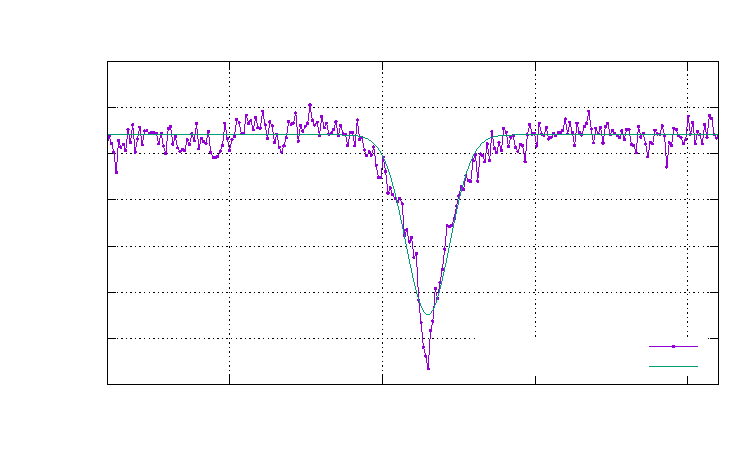
\includegraphics[width={360.00bp},height={216.00bp}]{29488-A5_gauss}}%
    \gplfronttext
  \end{picture}%
\endgroup
}
  \caption{} \label{fig:4b}
\end{figure}
\begin{figure}[h]
  \centering
  \resizebox{.5\textwidth}{!}{% GNUPLOT: LaTeX picture with Postscript
\begingroup
  \makeatletter
  \providecommand\color[2][]{%
    \GenericError{(gnuplot) \space\space\space\@spaces}{%
      Package color not loaded in conjunction with
      terminal option `colourtext'%
    }{See the gnuplot documentation for explanation.%
    }{Either use 'blacktext' in gnuplot or load the package
      color.sty in LaTeX.}%
    \renewcommand\color[2][]{}%
  }%
  \providecommand\includegraphics[2][]{%
    \GenericError{(gnuplot) \space\space\space\@spaces}{%
      Package graphicx or graphics not loaded%
    }{See the gnuplot documentation for explanation.%
    }{The gnuplot epslatex terminal needs graphicx.sty or graphics.sty.}%
    \renewcommand\includegraphics[2][]{}%
  }%
  \providecommand\rotatebox[2]{#2}%
  \@ifundefined{ifGPcolor}{%
    \newif\ifGPcolor
    \GPcolortrue
  }{}%
  \@ifundefined{ifGPblacktext}{%
    \newif\ifGPblacktext
    \GPblacktexttrue
  }{}%
  % define a \g@addto@macro without @ in the name:
  \let\gplgaddtomacro\g@addto@macro
  % define empty templates for all commands taking text:
  \gdef\gplbacktext{}%
  \gdef\gplfronttext{}%
  \makeatother
  \ifGPblacktext
    % no textcolor at all
    \def\colorrgb#1{}%
    \def\colorgray#1{}%
  \else
    % gray or color?
    \ifGPcolor
      \def\colorrgb#1{\color[rgb]{#1}}%
      \def\colorgray#1{\color[gray]{#1}}%
      \expandafter\def\csname LTw\endcsname{\color{white}}%
      \expandafter\def\csname LTb\endcsname{\color{black}}%
      \expandafter\def\csname LTa\endcsname{\color{black}}%
      \expandafter\def\csname LT0\endcsname{\color[rgb]{1,0,0}}%
      \expandafter\def\csname LT1\endcsname{\color[rgb]{0,1,0}}%
      \expandafter\def\csname LT2\endcsname{\color[rgb]{0,0,1}}%
      \expandafter\def\csname LT3\endcsname{\color[rgb]{1,0,1}}%
      \expandafter\def\csname LT4\endcsname{\color[rgb]{0,1,1}}%
      \expandafter\def\csname LT5\endcsname{\color[rgb]{1,1,0}}%
      \expandafter\def\csname LT6\endcsname{\color[rgb]{0,0,0}}%
      \expandafter\def\csname LT7\endcsname{\color[rgb]{1,0.3,0}}%
      \expandafter\def\csname LT8\endcsname{\color[rgb]{0.5,0.5,0.5}}%
    \else
      % gray
      \def\colorrgb#1{\color{black}}%
      \def\colorgray#1{\color[gray]{#1}}%
      \expandafter\def\csname LTw\endcsname{\color{white}}%
      \expandafter\def\csname LTb\endcsname{\color{black}}%
      \expandafter\def\csname LTa\endcsname{\color{black}}%
      \expandafter\def\csname LT0\endcsname{\color{black}}%
      \expandafter\def\csname LT1\endcsname{\color{black}}%
      \expandafter\def\csname LT2\endcsname{\color{black}}%
      \expandafter\def\csname LT3\endcsname{\color{black}}%
      \expandafter\def\csname LT4\endcsname{\color{black}}%
      \expandafter\def\csname LT5\endcsname{\color{black}}%
      \expandafter\def\csname LT6\endcsname{\color{black}}%
      \expandafter\def\csname LT7\endcsname{\color{black}}%
      \expandafter\def\csname LT8\endcsname{\color{black}}%
    \fi
  \fi
    \setlength{\unitlength}{0.0500bp}%
    \ifx\gptboxheight\undefined%
      \newlength{\gptboxheight}%
      \newlength{\gptboxwidth}%
      \newsavebox{\gptboxtext}%
    \fi%
    \setlength{\fboxrule}{0.5pt}%
    \setlength{\fboxsep}{1pt}%
    \definecolor{tbcol}{rgb}{1,1,1}%
\begin{picture}(7200.00,4320.00)%
    \gplgaddtomacro\gplbacktext{%
      \csname LTb\endcsname%%
      \put(1123,619){\makebox(0,0)[r]{\strut{}$635\cdot10^{-9}$}}%
      \csname LTb\endcsname%%
      \put(1123,963){\makebox(0,0)[r]{\strut{}$640\cdot10^{-9}$}}%
      \csname LTb\endcsname%%
      \put(1123,1308){\makebox(0,0)[r]{\strut{}$645\cdot10^{-9}$}}%
      \csname LTb\endcsname%%
      \put(1123,1652){\makebox(0,0)[r]{\strut{}$650\cdot10^{-9}$}}%
      \csname LTb\endcsname%%
      \put(1123,1997){\makebox(0,0)[r]{\strut{}$655\cdot10^{-9}$}}%
      \csname LTb\endcsname%%
      \put(1123,2341){\makebox(0,0)[r]{\strut{}$660\cdot10^{-9}$}}%
      \csname LTb\endcsname%%
      \put(1123,2686){\makebox(0,0)[r]{\strut{}$665\cdot10^{-9}$}}%
      \csname LTb\endcsname%%
      \put(1123,3030){\makebox(0,0)[r]{\strut{}$670\cdot10^{-9}$}}%
      \csname LTb\endcsname%%
      \put(1123,3374){\makebox(0,0)[r]{\strut{}$675\cdot10^{-9}$}}%
      \csname LTb\endcsname%%
      \put(1123,3719){\makebox(0,0)[r]{\strut{}$680\cdot10^{-9}$}}%
      \csname LTb\endcsname%%
      \put(1221,425){\makebox(0,0){\strut{}$50$}}%
      \csname LTb\endcsname%%
      \put(1736,425){\makebox(0,0){\strut{}$100$}}%
      \csname LTb\endcsname%%
      \put(2251,425){\makebox(0,0){\strut{}$150$}}%
      \csname LTb\endcsname%%
      \put(2766,425){\makebox(0,0){\strut{}$200$}}%
      \csname LTb\endcsname%%
      \put(3281,425){\makebox(0,0){\strut{}$250$}}%
      \csname LTb\endcsname%%
      \put(3796,425){\makebox(0,0){\strut{}$300$}}%
      \csname LTb\endcsname%%
      \put(4311,425){\makebox(0,0){\strut{}$350$}}%
      \csname LTb\endcsname%%
      \put(4826,425){\makebox(0,0){\strut{}$400$}}%
      \csname LTb\endcsname%%
      \put(5341,425){\makebox(0,0){\strut{}$450$}}%
      \csname LTb\endcsname%%
      \put(5856,425){\makebox(0,0){\strut{}$500$}}%
      \csname LTb\endcsname%%
      \put(6371,425){\makebox(0,0){\strut{}$550$}}%
      \csname LTb\endcsname%%
      \put(6886,425){\makebox(0,0){\strut{}$600$}}%
    }%
    \gplgaddtomacro\gplfronttext{%
      \csname LTb\endcsname%%
      \put(170,2169){\rotatebox{-270}{\makebox(0,0){\strut{}Wellenlänge $\lambda/\SI{}{m}$}}}%
      \csname LTb\endcsname%%
      \put(4053,135){\makebox(0,0){\strut{}Pixelkoordinate$/\textrm{Pixel}$}}%
      \csname LTb\endcsname%%
      \put(6123,3545){\makebox(0,0)[r]{\strut{}Datenpunkte}}%
      \csname LTb\endcsname%%
      \put(6123,3351){\makebox(0,0)[r]{\strut{}Anpassung $\lambda_\text{f}(x)$}}%
      \csname LTb\endcsname%%
      \put(4053,4009){\makebox(0,0){\strut{}Kalibraiton des 29488-A5 Spektrums mit $\chi^2/\textrm{ddof}=\SI{1.69E-02}{}$}}%
    }%
    \gplbacktext
    \put(0,0){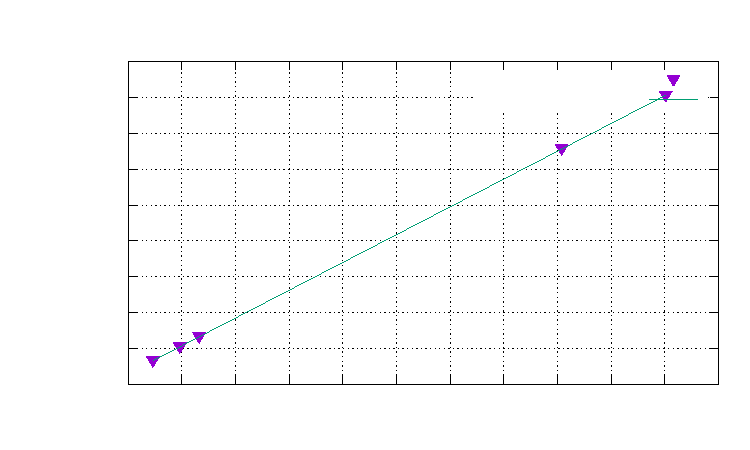
\includegraphics[width={360.00bp},height={216.00bp}]{29488-A5_kali}}%
    \gplfronttext
  \end{picture}%
\endgroup
}
  \caption{} \label{fig:4c}
\end{figure}
\begin{figure}[h]
  \centering
  \resizebox{.5\textwidth}{!}{% GNUPLOT: LaTeX picture with Postscript
\begingroup
  \makeatletter
  \providecommand\color[2][]{%
    \GenericError{(gnuplot) \space\space\space\@spaces}{%
      Package color not loaded in conjunction with
      terminal option `colourtext'%
    }{See the gnuplot documentation for explanation.%
    }{Either use 'blacktext' in gnuplot or load the package
      color.sty in LaTeX.}%
    \renewcommand\color[2][]{}%
  }%
  \providecommand\includegraphics[2][]{%
    \GenericError{(gnuplot) \space\space\space\@spaces}{%
      Package graphicx or graphics not loaded%
    }{See the gnuplot documentation for explanation.%
    }{The gnuplot epslatex terminal needs graphicx.sty or graphics.sty.}%
    \renewcommand\includegraphics[2][]{}%
  }%
  \providecommand\rotatebox[2]{#2}%
  \@ifundefined{ifGPcolor}{%
    \newif\ifGPcolor
    \GPcolortrue
  }{}%
  \@ifundefined{ifGPblacktext}{%
    \newif\ifGPblacktext
    \GPblacktexttrue
  }{}%
  % define a \g@addto@macro without @ in the name:
  \let\gplgaddtomacro\g@addto@macro
  % define empty templates for all commands taking text:
  \gdef\gplbacktext{}%
  \gdef\gplfronttext{}%
  \makeatother
  \ifGPblacktext
    % no textcolor at all
    \def\colorrgb#1{}%
    \def\colorgray#1{}%
  \else
    % gray or color?
    \ifGPcolor
      \def\colorrgb#1{\color[rgb]{#1}}%
      \def\colorgray#1{\color[gray]{#1}}%
      \expandafter\def\csname LTw\endcsname{\color{white}}%
      \expandafter\def\csname LTb\endcsname{\color{black}}%
      \expandafter\def\csname LTa\endcsname{\color{black}}%
      \expandafter\def\csname LT0\endcsname{\color[rgb]{1,0,0}}%
      \expandafter\def\csname LT1\endcsname{\color[rgb]{0,1,0}}%
      \expandafter\def\csname LT2\endcsname{\color[rgb]{0,0,1}}%
      \expandafter\def\csname LT3\endcsname{\color[rgb]{1,0,1}}%
      \expandafter\def\csname LT4\endcsname{\color[rgb]{0,1,1}}%
      \expandafter\def\csname LT5\endcsname{\color[rgb]{1,1,0}}%
      \expandafter\def\csname LT6\endcsname{\color[rgb]{0,0,0}}%
      \expandafter\def\csname LT7\endcsname{\color[rgb]{1,0.3,0}}%
      \expandafter\def\csname LT8\endcsname{\color[rgb]{0.5,0.5,0.5}}%
    \else
      % gray
      \def\colorrgb#1{\color{black}}%
      \def\colorgray#1{\color[gray]{#1}}%
      \expandafter\def\csname LTw\endcsname{\color{white}}%
      \expandafter\def\csname LTb\endcsname{\color{black}}%
      \expandafter\def\csname LTa\endcsname{\color{black}}%
      \expandafter\def\csname LT0\endcsname{\color{black}}%
      \expandafter\def\csname LT1\endcsname{\color{black}}%
      \expandafter\def\csname LT2\endcsname{\color{black}}%
      \expandafter\def\csname LT3\endcsname{\color{black}}%
      \expandafter\def\csname LT4\endcsname{\color{black}}%
      \expandafter\def\csname LT5\endcsname{\color{black}}%
      \expandafter\def\csname LT6\endcsname{\color{black}}%
      \expandafter\def\csname LT7\endcsname{\color{black}}%
      \expandafter\def\csname LT8\endcsname{\color{black}}%
    \fi
  \fi
    \setlength{\unitlength}{0.0500bp}%
    \ifx\gptboxheight\undefined%
      \newlength{\gptboxheight}%
      \newlength{\gptboxwidth}%
      \newsavebox{\gptboxtext}%
    \fi%
    \setlength{\fboxrule}{0.5pt}%
    \setlength{\fboxsep}{1pt}%
    \definecolor{tbcol}{rgb}{1,1,1}%
\begin{picture}(7200.00,4320.00)%
    \gplgaddtomacro\gplbacktext{%
      \csname LTb\endcsname%%
      \put(1123,619){\makebox(0,0)[r]{\strut{}300\cdot10^{-3}}}%
      \csname LTb\endcsname%%
      \put(1123,1062){\makebox(0,0)[r]{\strut{}400\cdot10^{-3}}}%
      \csname LTb\endcsname%%
      \put(1123,1505){\makebox(0,0)[r]{\strut{}500\cdot10^{-3}}}%
      \csname LTb\endcsname%%
      \put(1123,1947){\makebox(0,0)[r]{\strut{}600\cdot10^{-3}}}%
      \csname LTb\endcsname%%
      \put(1123,2390){\makebox(0,0)[r]{\strut{}700\cdot10^{-3}}}%
      \csname LTb\endcsname%%
      \put(1123,2833){\makebox(0,0)[r]{\strut{}800\cdot10^{-3}}}%
      \csname LTb\endcsname%%
      \put(1123,3276){\makebox(0,0)[r]{\strut{}900\cdot10^{-3}}}%
      \csname LTb\endcsname%%
      \put(1123,3719){\makebox(0,0)[r]{\strut{}1\cdot10^{0}}}%
      \csname LTb\endcsname%%
      \put(1221,425){\makebox(0,0){\strut{}$0$}}%
      \csname LTb\endcsname%%
      \put(1929,425){\makebox(0,0){\strut{}$100$}}%
      \csname LTb\endcsname%%
      \put(2637,425){\makebox(0,0){\strut{}$200$}}%
      \csname LTb\endcsname%%
      \put(3345,425){\makebox(0,0){\strut{}$300$}}%
      \csname LTb\endcsname%%
      \put(4053,425){\makebox(0,0){\strut{}$400$}}%
      \csname LTb\endcsname%%
      \put(4761,425){\makebox(0,0){\strut{}$500$}}%
      \csname LTb\endcsname%%
      \put(5470,425){\makebox(0,0){\strut{}$600$}}%
      \csname LTb\endcsname%%
      \put(6178,425){\makebox(0,0){\strut{}$700$}}%
      \csname LTb\endcsname%%
      \put(6886,425){\makebox(0,0){\strut{}$800$}}%
    }%
    \gplgaddtomacro\gplfronttext{%
      \csname LTb\endcsname%%
      \put(6123,3545){\makebox(0,0)[r]{\strut{}60179-A1}}%
      \csname LTb\endcsname%%
      \put(6123,3351){\makebox(0,0)[r]{\strut{}Kalibrationslampe}}%
      \csname LTb\endcsname%%
      \put(170,2169){\rotatebox{-270.00}{\makebox(0,0){\strut{}Amplitude$/\textrm{a.u.}$}}}%
      \csname LTb\endcsname%%
      \put(4053,135){\makebox(0,0){\strut{}Pixelkoordinate$/\textrm{Pixel}$}}%
      \csname LTb\endcsname%%
      \put(4053,4009){\makebox(0,0){\strut{}Spektrum}}%
    }%
    \gplbacktext
    \put(0,0){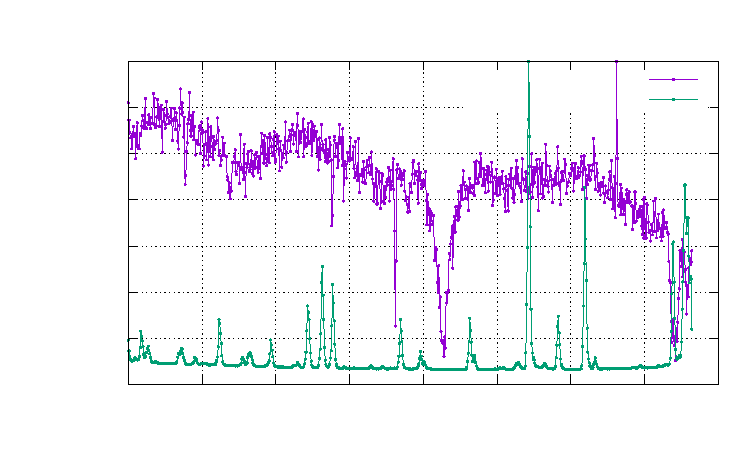
\includegraphics[width={360.00bp},height={216.00bp}]{60179-A1_data}}%
    \gplfronttext
  \end{picture}%
\endgroup
}
  \caption{} \label{fig:5a}
\end{figure}
\begin{figure}[h]
  \centering
  \resizebox{.5\textwidth}{!}{% GNUPLOT: LaTeX picture with Postscript
\begingroup
  \makeatletter
  \providecommand\color[2][]{%
    \GenericError{(gnuplot) \space\space\space\@spaces}{%
      Package color not loaded in conjunction with
      terminal option `colourtext'%
    }{See the gnuplot documentation for explanation.%
    }{Either use 'blacktext' in gnuplot or load the package
      color.sty in LaTeX.}%
    \renewcommand\color[2][]{}%
  }%
  \providecommand\includegraphics[2][]{%
    \GenericError{(gnuplot) \space\space\space\@spaces}{%
      Package graphicx or graphics not loaded%
    }{See the gnuplot documentation for explanation.%
    }{The gnuplot epslatex terminal needs graphicx.sty or graphics.sty.}%
    \renewcommand\includegraphics[2][]{}%
  }%
  \providecommand\rotatebox[2]{#2}%
  \@ifundefined{ifGPcolor}{%
    \newif\ifGPcolor
    \GPcolortrue
  }{}%
  \@ifundefined{ifGPblacktext}{%
    \newif\ifGPblacktext
    \GPblacktexttrue
  }{}%
  % define a \g@addto@macro without @ in the name:
  \let\gplgaddtomacro\g@addto@macro
  % define empty templates for all commands taking text:
  \gdef\gplbacktext{}%
  \gdef\gplfronttext{}%
  \makeatother
  \ifGPblacktext
    % no textcolor at all
    \def\colorrgb#1{}%
    \def\colorgray#1{}%
  \else
    % gray or color?
    \ifGPcolor
      \def\colorrgb#1{\color[rgb]{#1}}%
      \def\colorgray#1{\color[gray]{#1}}%
      \expandafter\def\csname LTw\endcsname{\color{white}}%
      \expandafter\def\csname LTb\endcsname{\color{black}}%
      \expandafter\def\csname LTa\endcsname{\color{black}}%
      \expandafter\def\csname LT0\endcsname{\color[rgb]{1,0,0}}%
      \expandafter\def\csname LT1\endcsname{\color[rgb]{0,1,0}}%
      \expandafter\def\csname LT2\endcsname{\color[rgb]{0,0,1}}%
      \expandafter\def\csname LT3\endcsname{\color[rgb]{1,0,1}}%
      \expandafter\def\csname LT4\endcsname{\color[rgb]{0,1,1}}%
      \expandafter\def\csname LT5\endcsname{\color[rgb]{1,1,0}}%
      \expandafter\def\csname LT6\endcsname{\color[rgb]{0,0,0}}%
      \expandafter\def\csname LT7\endcsname{\color[rgb]{1,0.3,0}}%
      \expandafter\def\csname LT8\endcsname{\color[rgb]{0.5,0.5,0.5}}%
    \else
      % gray
      \def\colorrgb#1{\color{black}}%
      \def\colorgray#1{\color[gray]{#1}}%
      \expandafter\def\csname LTw\endcsname{\color{white}}%
      \expandafter\def\csname LTb\endcsname{\color{black}}%
      \expandafter\def\csname LTa\endcsname{\color{black}}%
      \expandafter\def\csname LT0\endcsname{\color{black}}%
      \expandafter\def\csname LT1\endcsname{\color{black}}%
      \expandafter\def\csname LT2\endcsname{\color{black}}%
      \expandafter\def\csname LT3\endcsname{\color{black}}%
      \expandafter\def\csname LT4\endcsname{\color{black}}%
      \expandafter\def\csname LT5\endcsname{\color{black}}%
      \expandafter\def\csname LT6\endcsname{\color{black}}%
      \expandafter\def\csname LT7\endcsname{\color{black}}%
      \expandafter\def\csname LT8\endcsname{\color{black}}%
    \fi
  \fi
    \setlength{\unitlength}{0.0500bp}%
    \ifx\gptboxheight\undefined%
      \newlength{\gptboxheight}%
      \newlength{\gptboxwidth}%
      \newsavebox{\gptboxtext}%
    \fi%
    \setlength{\fboxrule}{0.5pt}%
    \setlength{\fboxsep}{1pt}%
    \definecolor{tbcol}{rgb}{1,1,1}%
\begin{picture}(7200.00,4320.00)%
    \gplgaddtomacro\gplbacktext{%
      \csname LTb\endcsname%%
      \put(927,619){\makebox(0,0)[r]{\strut{}4\cdot10^{3}}}%
      \csname LTb\endcsname%%
      \put(927,1062){\makebox(0,0)[r]{\strut{}5\cdot10^{3}}}%
      \csname LTb\endcsname%%
      \put(927,1505){\makebox(0,0)[r]{\strut{}6\cdot10^{3}}}%
      \csname LTb\endcsname%%
      \put(927,1947){\makebox(0,0)[r]{\strut{}7\cdot10^{3}}}%
      \csname LTb\endcsname%%
      \put(927,2390){\makebox(0,0)[r]{\strut{}8\cdot10^{3}}}%
      \csname LTb\endcsname%%
      \put(927,2833){\makebox(0,0)[r]{\strut{}9\cdot10^{3}}}%
      \csname LTb\endcsname%%
      \put(927,3276){\makebox(0,0)[r]{\strut{}10\cdot10^{3}}}%
      \csname LTb\endcsname%%
      \put(927,3719){\makebox(0,0)[r]{\strut{}11\cdot10^{3}}}%
      \csname LTb\endcsname%%
      \put(2197,425){\makebox(0,0){\strut{}650\cdot10^{-9}}}%
      \csname LTb\endcsname%%
      \put(3662,425){\makebox(0,0){\strut{}655\cdot10^{-9}}}%
      \csname LTb\endcsname%%
      \put(5128,425){\makebox(0,0){\strut{}660\cdot10^{-9}}}%
      \csname LTb\endcsname%%
      \put(6593,425){\makebox(0,0){\strut{}665\cdot10^{-9}}}%
    }%
    \gplgaddtomacro\gplfronttext{%
      \csname LTb\endcsname%%
      \put(6123,986){\makebox(0,0)[r]{\strut{}Datenpunkte}}%
      \csname LTb\endcsname%%
      \put(6123,793){\makebox(0,0)[r]{\strut{}Anpassung $G_\text{f}(x)$}}%
      \csname LTb\endcsname%%
      \put(170,2169){\rotatebox{-270.00}{\makebox(0,0){\strut{}Amplitude$/\textrm{a.u.}$}}}%
      \csname LTb\endcsname%%
      \put(3955,135){\makebox(0,0){\strut{}Wellenlänge $\lambda/\SI{}{m}$}}%
      \csname LTb\endcsname%%
      \put(3955,4009){\makebox(0,0){\strut{}H$\alpha$(\SI{656}{nm})-Linie von 60179-A1 mit $\chi^2/\textrm{ddof}=\SI{2.32E-01}{}$}}%
    }%
    \gplbacktext
    \put(0,0){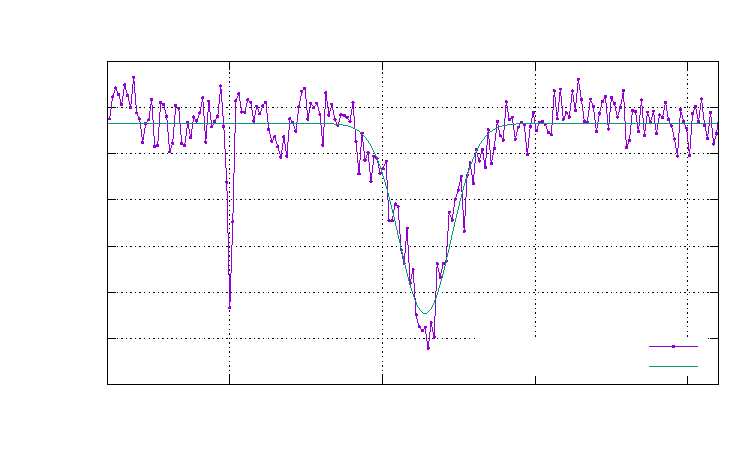
\includegraphics[width={360.00bp},height={216.00bp}]{60179-A1_gauss}}%
    \gplfronttext
  \end{picture}%
\endgroup
}
  \caption{} \label{fig:5b}
\end{figure}
\begin{figure}[h]
  \centering
  \resizebox{.5\textwidth}{!}{% GNUPLOT: LaTeX picture with Postscript
\begingroup
  \makeatletter
  \providecommand\color[2][]{%
    \GenericError{(gnuplot) \space\space\space\@spaces}{%
      Package color not loaded in conjunction with
      terminal option `colourtext'%
    }{See the gnuplot documentation for explanation.%
    }{Either use 'blacktext' in gnuplot or load the package
      color.sty in LaTeX.}%
    \renewcommand\color[2][]{}%
  }%
  \providecommand\includegraphics[2][]{%
    \GenericError{(gnuplot) \space\space\space\@spaces}{%
      Package graphicx or graphics not loaded%
    }{See the gnuplot documentation for explanation.%
    }{The gnuplot epslatex terminal needs graphicx.sty or graphics.sty.}%
    \renewcommand\includegraphics[2][]{}%
  }%
  \providecommand\rotatebox[2]{#2}%
  \@ifundefined{ifGPcolor}{%
    \newif\ifGPcolor
    \GPcolortrue
  }{}%
  \@ifundefined{ifGPblacktext}{%
    \newif\ifGPblacktext
    \GPblacktexttrue
  }{}%
  % define a \g@addto@macro without @ in the name:
  \let\gplgaddtomacro\g@addto@macro
  % define empty templates for all commands taking text:
  \gdef\gplbacktext{}%
  \gdef\gplfronttext{}%
  \makeatother
  \ifGPblacktext
    % no textcolor at all
    \def\colorrgb#1{}%
    \def\colorgray#1{}%
  \else
    % gray or color?
    \ifGPcolor
      \def\colorrgb#1{\color[rgb]{#1}}%
      \def\colorgray#1{\color[gray]{#1}}%
      \expandafter\def\csname LTw\endcsname{\color{white}}%
      \expandafter\def\csname LTb\endcsname{\color{black}}%
      \expandafter\def\csname LTa\endcsname{\color{black}}%
      \expandafter\def\csname LT0\endcsname{\color[rgb]{1,0,0}}%
      \expandafter\def\csname LT1\endcsname{\color[rgb]{0,1,0}}%
      \expandafter\def\csname LT2\endcsname{\color[rgb]{0,0,1}}%
      \expandafter\def\csname LT3\endcsname{\color[rgb]{1,0,1}}%
      \expandafter\def\csname LT4\endcsname{\color[rgb]{0,1,1}}%
      \expandafter\def\csname LT5\endcsname{\color[rgb]{1,1,0}}%
      \expandafter\def\csname LT6\endcsname{\color[rgb]{0,0,0}}%
      \expandafter\def\csname LT7\endcsname{\color[rgb]{1,0.3,0}}%
      \expandafter\def\csname LT8\endcsname{\color[rgb]{0.5,0.5,0.5}}%
    \else
      % gray
      \def\colorrgb#1{\color{black}}%
      \def\colorgray#1{\color[gray]{#1}}%
      \expandafter\def\csname LTw\endcsname{\color{white}}%
      \expandafter\def\csname LTb\endcsname{\color{black}}%
      \expandafter\def\csname LTa\endcsname{\color{black}}%
      \expandafter\def\csname LT0\endcsname{\color{black}}%
      \expandafter\def\csname LT1\endcsname{\color{black}}%
      \expandafter\def\csname LT2\endcsname{\color{black}}%
      \expandafter\def\csname LT3\endcsname{\color{black}}%
      \expandafter\def\csname LT4\endcsname{\color{black}}%
      \expandafter\def\csname LT5\endcsname{\color{black}}%
      \expandafter\def\csname LT6\endcsname{\color{black}}%
      \expandafter\def\csname LT7\endcsname{\color{black}}%
      \expandafter\def\csname LT8\endcsname{\color{black}}%
    \fi
  \fi
    \setlength{\unitlength}{0.0500bp}%
    \ifx\gptboxheight\undefined%
      \newlength{\gptboxheight}%
      \newlength{\gptboxwidth}%
      \newsavebox{\gptboxtext}%
    \fi%
    \setlength{\fboxrule}{0.5pt}%
    \setlength{\fboxsep}{1pt}%
    \definecolor{tbcol}{rgb}{1,1,1}%
\begin{picture}(7200.00,4320.00)%
    \gplgaddtomacro\gplbacktext{%
      \csname LTb\endcsname%%
      \put(1123,619){\makebox(0,0)[r]{\strut{}$635\cdot10^{-9}$}}%
      \csname LTb\endcsname%%
      \put(1123,963){\makebox(0,0)[r]{\strut{}$640\cdot10^{-9}$}}%
      \csname LTb\endcsname%%
      \put(1123,1308){\makebox(0,0)[r]{\strut{}$645\cdot10^{-9}$}}%
      \csname LTb\endcsname%%
      \put(1123,1652){\makebox(0,0)[r]{\strut{}$650\cdot10^{-9}$}}%
      \csname LTb\endcsname%%
      \put(1123,1997){\makebox(0,0)[r]{\strut{}$655\cdot10^{-9}$}}%
      \csname LTb\endcsname%%
      \put(1123,2341){\makebox(0,0)[r]{\strut{}$660\cdot10^{-9}$}}%
      \csname LTb\endcsname%%
      \put(1123,2686){\makebox(0,0)[r]{\strut{}$665\cdot10^{-9}$}}%
      \csname LTb\endcsname%%
      \put(1123,3030){\makebox(0,0)[r]{\strut{}$670\cdot10^{-9}$}}%
      \csname LTb\endcsname%%
      \put(1123,3374){\makebox(0,0)[r]{\strut{}$675\cdot10^{-9}$}}%
      \csname LTb\endcsname%%
      \put(1123,3719){\makebox(0,0)[r]{\strut{}$680\cdot10^{-9}$}}%
      \csname LTb\endcsname%%
      \put(1221,425){\makebox(0,0){\strut{}$200$}}%
      \csname LTb\endcsname%%
      \put(1850,425){\makebox(0,0){\strut{}$250$}}%
      \csname LTb\endcsname%%
      \put(2480,425){\makebox(0,0){\strut{}$300$}}%
      \csname LTb\endcsname%%
      \put(3109,425){\makebox(0,0){\strut{}$350$}}%
      \csname LTb\endcsname%%
      \put(3739,425){\makebox(0,0){\strut{}$400$}}%
      \csname LTb\endcsname%%
      \put(4368,425){\makebox(0,0){\strut{}$450$}}%
      \csname LTb\endcsname%%
      \put(4997,425){\makebox(0,0){\strut{}$500$}}%
      \csname LTb\endcsname%%
      \put(5627,425){\makebox(0,0){\strut{}$550$}}%
      \csname LTb\endcsname%%
      \put(6256,425){\makebox(0,0){\strut{}$600$}}%
      \csname LTb\endcsname%%
      \put(6886,425){\makebox(0,0){\strut{}$650$}}%
    }%
    \gplgaddtomacro\gplfronttext{%
      \csname LTb\endcsname%%
      \put(170,2169){\rotatebox{-270}{\makebox(0,0){\strut{}Wellenlänge $\lambda/\SI{}{m}$}}}%
      \csname LTb\endcsname%%
      \put(4053,135){\makebox(0,0){\strut{}Pixelkoordinate$/\textrm{Pixel}$}}%
      \csname LTb\endcsname%%
      \put(6123,3545){\makebox(0,0)[r]{\strut{}Datenpunkte}}%
      \csname LTb\endcsname%%
      \put(6123,3351){\makebox(0,0)[r]{\strut{}Anpassung $\lambda_\text{f}(x)$}}%
      \csname LTb\endcsname%%
      \put(4053,4009){\makebox(0,0){\strut{}Kalibraiton des 60179-A1 Spektrums mit $\chi^2/\textrm{ddof}=\SI{1.45E-02}{}$}}%
    }%
    \gplbacktext
    \put(0,0){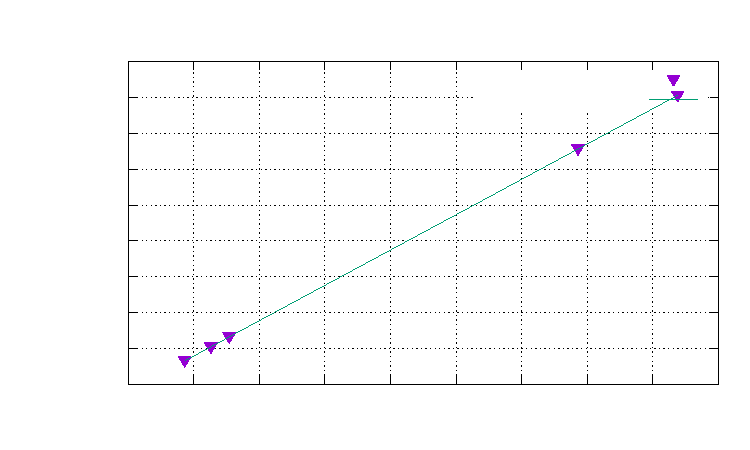
\includegraphics[width={360.00bp},height={216.00bp}]{60179-A1_kali}}%
    \gplfronttext
  \end{picture}%
\endgroup
}
  \caption{} \label{fig:5c}
\end{figure}
\begin{figure}[h]
  \centering
  \resizebox{.5\textwidth}{!}{\input{äquivalenzbreiten.tex}}
  \caption{Äquivalenzbreiten} \label{fig:äquivalenzbreiten}
\end{figure}
\begin{figure}[h]
  \centering
  \resizebox{.5\textwidth}{!}{% GNUPLOT: LaTeX picture with Postscript
\begingroup
  \makeatletter
  \providecommand\color[2][]{%
    \GenericError{(gnuplot) \space\space\space\@spaces}{%
      Package color not loaded in conjunction with
      terminal option `colourtext'%
    }{See the gnuplot documentation for explanation.%
    }{Either use 'blacktext' in gnuplot or load the package
      color.sty in LaTeX.}%
    \renewcommand\color[2][]{}%
  }%
  \providecommand\includegraphics[2][]{%
    \GenericError{(gnuplot) \space\space\space\@spaces}{%
      Package graphicx or graphics not loaded%
    }{See the gnuplot documentation for explanation.%
    }{The gnuplot epslatex terminal needs graphicx.sty or graphics.sty.}%
    \renewcommand\includegraphics[2][]{}%
  }%
  \providecommand\rotatebox[2]{#2}%
  \@ifundefined{ifGPcolor}{%
    \newif\ifGPcolor
    \GPcolortrue
  }{}%
  \@ifundefined{ifGPblacktext}{%
    \newif\ifGPblacktext
    \GPblacktexttrue
  }{}%
  % define a \g@addto@macro without @ in the name:
  \let\gplgaddtomacro\g@addto@macro
  % define empty templates for all commands taking text:
  \gdef\gplbacktext{}%
  \gdef\gplfronttext{}%
  \makeatother
  \ifGPblacktext
    % no textcolor at all
    \def\colorrgb#1{}%
    \def\colorgray#1{}%
  \else
    % gray or color?
    \ifGPcolor
      \def\colorrgb#1{\color[rgb]{#1}}%
      \def\colorgray#1{\color[gray]{#1}}%
      \expandafter\def\csname LTw\endcsname{\color{white}}%
      \expandafter\def\csname LTb\endcsname{\color{black}}%
      \expandafter\def\csname LTa\endcsname{\color{black}}%
      \expandafter\def\csname LT0\endcsname{\color[rgb]{1,0,0}}%
      \expandafter\def\csname LT1\endcsname{\color[rgb]{0,1,0}}%
      \expandafter\def\csname LT2\endcsname{\color[rgb]{0,0,1}}%
      \expandafter\def\csname LT3\endcsname{\color[rgb]{1,0,1}}%
      \expandafter\def\csname LT4\endcsname{\color[rgb]{0,1,1}}%
      \expandafter\def\csname LT5\endcsname{\color[rgb]{1,1,0}}%
      \expandafter\def\csname LT6\endcsname{\color[rgb]{0,0,0}}%
      \expandafter\def\csname LT7\endcsname{\color[rgb]{1,0.3,0}}%
      \expandafter\def\csname LT8\endcsname{\color[rgb]{0.5,0.5,0.5}}%
    \else
      % gray
      \def\colorrgb#1{\color{black}}%
      \def\colorgray#1{\color[gray]{#1}}%
      \expandafter\def\csname LTw\endcsname{\color{white}}%
      \expandafter\def\csname LTb\endcsname{\color{black}}%
      \expandafter\def\csname LTa\endcsname{\color{black}}%
      \expandafter\def\csname LT0\endcsname{\color{black}}%
      \expandafter\def\csname LT1\endcsname{\color{black}}%
      \expandafter\def\csname LT2\endcsname{\color{black}}%
      \expandafter\def\csname LT3\endcsname{\color{black}}%
      \expandafter\def\csname LT4\endcsname{\color{black}}%
      \expandafter\def\csname LT5\endcsname{\color{black}}%
      \expandafter\def\csname LT6\endcsname{\color{black}}%
      \expandafter\def\csname LT7\endcsname{\color{black}}%
      \expandafter\def\csname LT8\endcsname{\color{black}}%
    \fi
  \fi
    \setlength{\unitlength}{0.0500bp}%
    \ifx\gptboxheight\undefined%
      \newlength{\gptboxheight}%
      \newlength{\gptboxwidth}%
      \newsavebox{\gptboxtext}%
    \fi%
    \setlength{\fboxrule}{0.5pt}%
    \setlength{\fboxsep}{1pt}%
    \definecolor{tbcol}{rgb}{1,1,1}%
\begin{picture}(7200.00,4320.00)%
    \gplgaddtomacro\gplbacktext{%
      \csname LTb\endcsname%%
      \put(1025,619){\makebox(0,0)[r]{\strut{}0\cdot10^{0}}}%
      \csname LTb\endcsname%%
      \put(1025,963){\makebox(0,0)[r]{\strut{}100\cdot10^{3}}}%
      \csname LTb\endcsname%%
      \put(1025,1308){\makebox(0,0)[r]{\strut{}200\cdot10^{3}}}%
      \csname LTb\endcsname%%
      \put(1025,1652){\makebox(0,0)[r]{\strut{}300\cdot10^{3}}}%
      \csname LTb\endcsname%%
      \put(1025,1997){\makebox(0,0)[r]{\strut{}400\cdot10^{3}}}%
      \csname LTb\endcsname%%
      \put(1025,2341){\makebox(0,0)[r]{\strut{}500\cdot10^{3}}}%
      \csname LTb\endcsname%%
      \put(1025,2686){\makebox(0,0)[r]{\strut{}600\cdot10^{3}}}%
      \csname LTb\endcsname%%
      \put(1025,3030){\makebox(0,0)[r]{\strut{}700\cdot10^{3}}}%
      \csname LTb\endcsname%%
      \put(1025,3374){\makebox(0,0)[r]{\strut{}800\cdot10^{3}}}%
      \csname LTb\endcsname%%
      \put(1025,3719){\makebox(0,0)[r]{\strut{}900\cdot10^{3}}}%
      \csname LTb\endcsname%%
      \put(1123,425){\makebox(0,0){\strut{}630\cdot10^{-9}}}%
      \csname LTb\endcsname%%
      \put(2084,425){\makebox(0,0){\strut{}640\cdot10^{-9}}}%
      \csname LTb\endcsname%%
      \put(3044,425){\makebox(0,0){\strut{}650\cdot10^{-9}}}%
      \csname LTb\endcsname%%
      \put(4004,425){\makebox(0,0){\strut{}660\cdot10^{-9}}}%
      \csname LTb\endcsname%%
      \put(4965,425){\makebox(0,0){\strut{}670\cdot10^{-9}}}%
      \csname LTb\endcsname%%
      \put(5925,425){\makebox(0,0){\strut{}680\cdot10^{-9}}}%
      \csname LTb\endcsname%%
      \put(6886,425){\makebox(0,0){\strut{}690\cdot10^{-9}}}%
    }%
    \gplgaddtomacro\gplfronttext{%
      \csname LTb\endcsname%%
      \put(6123,3545){\makebox(0,0)[r]{\strut{}Datenpunkte}}%
      \csname LTb\endcsname%%
      \put(170,2169){\rotatebox{-270.00}{\makebox(0,0){\strut{}Amplitude$/\SI{}{a.u}$}}}%
      \csname LTb\endcsname%%
      \put(4004,135){\makebox(0,0){\strut{}Wellenlänge $\lambda/\SI{}{m}$}}%
      \csname LTb\endcsname%%
      \put(4004,4009){\makebox(0,0){\strut{}P-Cygni Spektrum}}%
    }%
    \gplbacktext
    \put(0,0){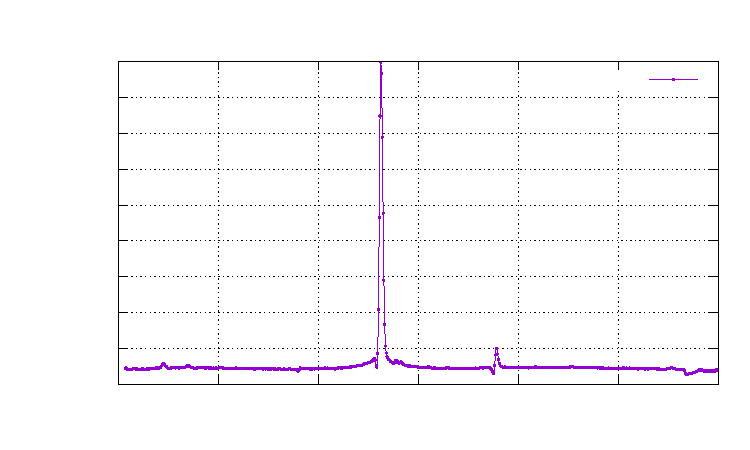
\includegraphics[width={360.00bp},height={216.00bp}]{P_Cygni_spectra}}%
    \gplfronttext
  \end{picture}%
\endgroup
}
  \caption{} \label{fig:pcygniSpektrum}
\end{figure}
\begin{figure}[h]
  \centering
  \resizebox{.5\textwidth}{!}{% GNUPLOT: LaTeX picture with Postscript
\begingroup
  \makeatletter
  \providecommand\color[2][]{%
    \GenericError{(gnuplot) \space\space\space\@spaces}{%
      Package color not loaded in conjunction with
      terminal option `colourtext'%
    }{See the gnuplot documentation for explanation.%
    }{Either use 'blacktext' in gnuplot or load the package
      color.sty in LaTeX.}%
    \renewcommand\color[2][]{}%
  }%
  \providecommand\includegraphics[2][]{%
    \GenericError{(gnuplot) \space\space\space\@spaces}{%
      Package graphicx or graphics not loaded%
    }{See the gnuplot documentation for explanation.%
    }{The gnuplot epslatex terminal needs graphicx.sty or graphics.sty.}%
    \renewcommand\includegraphics[2][]{}%
  }%
  \providecommand\rotatebox[2]{#2}%
  \@ifundefined{ifGPcolor}{%
    \newif\ifGPcolor
    \GPcolortrue
  }{}%
  \@ifundefined{ifGPblacktext}{%
    \newif\ifGPblacktext
    \GPblacktexttrue
  }{}%
  % define a \g@addto@macro without @ in the name:
  \let\gplgaddtomacro\g@addto@macro
  % define empty templates for all commands taking text:
  \gdef\gplbacktext{}%
  \gdef\gplfronttext{}%
  \makeatother
  \ifGPblacktext
    % no textcolor at all
    \def\colorrgb#1{}%
    \def\colorgray#1{}%
  \else
    % gray or color?
    \ifGPcolor
      \def\colorrgb#1{\color[rgb]{#1}}%
      \def\colorgray#1{\color[gray]{#1}}%
      \expandafter\def\csname LTw\endcsname{\color{white}}%
      \expandafter\def\csname LTb\endcsname{\color{black}}%
      \expandafter\def\csname LTa\endcsname{\color{black}}%
      \expandafter\def\csname LT0\endcsname{\color[rgb]{1,0,0}}%
      \expandafter\def\csname LT1\endcsname{\color[rgb]{0,1,0}}%
      \expandafter\def\csname LT2\endcsname{\color[rgb]{0,0,1}}%
      \expandafter\def\csname LT3\endcsname{\color[rgb]{1,0,1}}%
      \expandafter\def\csname LT4\endcsname{\color[rgb]{0,1,1}}%
      \expandafter\def\csname LT5\endcsname{\color[rgb]{1,1,0}}%
      \expandafter\def\csname LT6\endcsname{\color[rgb]{0,0,0}}%
      \expandafter\def\csname LT7\endcsname{\color[rgb]{1,0.3,0}}%
      \expandafter\def\csname LT8\endcsname{\color[rgb]{0.5,0.5,0.5}}%
    \else
      % gray
      \def\colorrgb#1{\color{black}}%
      \def\colorgray#1{\color[gray]{#1}}%
      \expandafter\def\csname LTw\endcsname{\color{white}}%
      \expandafter\def\csname LTb\endcsname{\color{black}}%
      \expandafter\def\csname LTa\endcsname{\color{black}}%
      \expandafter\def\csname LT0\endcsname{\color{black}}%
      \expandafter\def\csname LT1\endcsname{\color{black}}%
      \expandafter\def\csname LT2\endcsname{\color{black}}%
      \expandafter\def\csname LT3\endcsname{\color{black}}%
      \expandafter\def\csname LT4\endcsname{\color{black}}%
      \expandafter\def\csname LT5\endcsname{\color{black}}%
      \expandafter\def\csname LT6\endcsname{\color{black}}%
      \expandafter\def\csname LT7\endcsname{\color{black}}%
      \expandafter\def\csname LT8\endcsname{\color{black}}%
    \fi
  \fi
    \setlength{\unitlength}{0.0500bp}%
    \ifx\gptboxheight\undefined%
      \newlength{\gptboxheight}%
      \newlength{\gptboxwidth}%
      \newsavebox{\gptboxtext}%
    \fi%
    \setlength{\fboxrule}{0.5pt}%
    \setlength{\fboxsep}{1pt}%
    \definecolor{tbcol}{rgb}{1,1,1}%
\begin{picture}(7200.00,4320.00)%
    \gplgaddtomacro\gplbacktext{%
      \csname LTb\endcsname%%
      \put(927,619){\makebox(0,0)[r]{\strut{}36\cdot10^{3}}}%
      \csname LTb\endcsname%%
      \put(927,1135){\makebox(0,0)[r]{\strut{}38\cdot10^{3}}}%
      \csname LTb\endcsname%%
      \put(927,1652){\makebox(0,0)[r]{\strut{}40\cdot10^{3}}}%
      \csname LTb\endcsname%%
      \put(927,2169){\makebox(0,0)[r]{\strut{}42\cdot10^{3}}}%
      \csname LTb\endcsname%%
      \put(927,2686){\makebox(0,0)[r]{\strut{}44\cdot10^{3}}}%
      \csname LTb\endcsname%%
      \put(927,3202){\makebox(0,0)[r]{\strut{}46\cdot10^{3}}}%
      \csname LTb\endcsname%%
      \put(927,3719){\makebox(0,0)[r]{\strut{}48\cdot10^{3}}}%
      \csname LTb\endcsname%%
      \put(2127,425){\makebox(0,0){\strut{}647\cdot10^{-9}}}%
      \csname LTb\endcsname%%
      \put(3641,425){\makebox(0,0){\strut{}648\cdot10^{-9}}}%
      \csname LTb\endcsname%%
      \put(5155,425){\makebox(0,0){\strut{}649\cdot10^{-9}}}%
      \csname LTb\endcsname%%
      \put(6669,425){\makebox(0,0){\strut{}650\cdot10^{-9}}}%
    }%
    \gplgaddtomacro\gplfronttext{%
      \csname LTb\endcsname%%
      \put(6123,3545){\makebox(0,0)[r]{\strut{}Datenpunkte}}%
      \csname LTb\endcsname%%
      \put(6123,3351){\makebox(0,0)[r]{\strut{}Anpassung $G_\text{f}(x)$}}%
      \csname LTb\endcsname%%
      \put(170,2169){\rotatebox{-270.00}{\makebox(0,0){\strut{}Amplitude$/\textrm{a.u.}$}}}%
      \csname LTb\endcsname%%
      \put(3955,135){\makebox(0,0){\strut{}Wellenlänge $\lambda/\SI{}{m}$}}%
      \csname LTb\endcsname%%
      \put(3955,4009){\makebox(0,0){\strut{}H$\alpha$(\SI{656}{nm})-Linie von He2 mit $\chi^2/\textrm{ddof}=\SI{2.02E-01}{}$}}%
    }%
    \gplbacktext
    \put(0,0){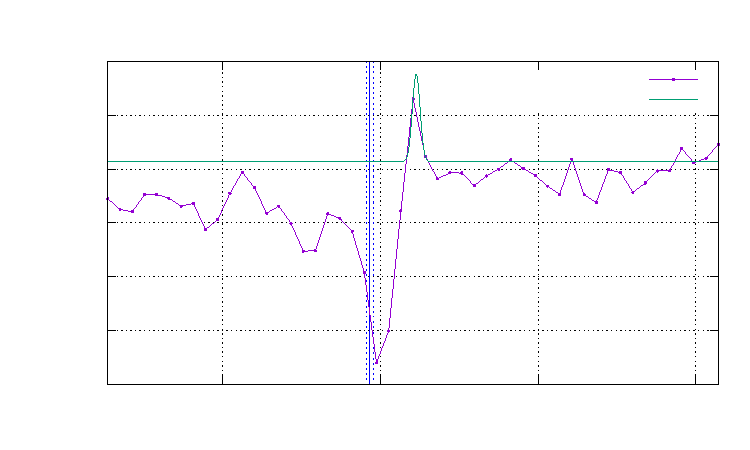
\includegraphics[width={360.00bp},height={216.00bp}]{P-Cygni_He2_gauss}}%
    \gplfronttext
  \end{picture}%
\endgroup
}
  \caption{} \label{fig:pcHe2}
\end{figure}
\begin{figure}[h]
  \centering
  \resizebox{.5\textwidth}{!}{% GNUPLOT: LaTeX picture with Postscript
\begingroup
  \makeatletter
  \providecommand\color[2][]{%
    \GenericError{(gnuplot) \space\space\space\@spaces}{%
      Package color not loaded in conjunction with
      terminal option `colourtext'%
    }{See the gnuplot documentation for explanation.%
    }{Either use 'blacktext' in gnuplot or load the package
      color.sty in LaTeX.}%
    \renewcommand\color[2][]{}%
  }%
  \providecommand\includegraphics[2][]{%
    \GenericError{(gnuplot) \space\space\space\@spaces}{%
      Package graphicx or graphics not loaded%
    }{See the gnuplot documentation for explanation.%
    }{The gnuplot epslatex terminal needs graphicx.sty or graphics.sty.}%
    \renewcommand\includegraphics[2][]{}%
  }%
  \providecommand\rotatebox[2]{#2}%
  \@ifundefined{ifGPcolor}{%
    \newif\ifGPcolor
    \GPcolortrue
  }{}%
  \@ifundefined{ifGPblacktext}{%
    \newif\ifGPblacktext
    \GPblacktexttrue
  }{}%
  % define a \g@addto@macro without @ in the name:
  \let\gplgaddtomacro\g@addto@macro
  % define empty templates for all commands taking text:
  \gdef\gplbacktext{}%
  \gdef\gplfronttext{}%
  \makeatother
  \ifGPblacktext
    % no textcolor at all
    \def\colorrgb#1{}%
    \def\colorgray#1{}%
  \else
    % gray or color?
    \ifGPcolor
      \def\colorrgb#1{\color[rgb]{#1}}%
      \def\colorgray#1{\color[gray]{#1}}%
      \expandafter\def\csname LTw\endcsname{\color{white}}%
      \expandafter\def\csname LTb\endcsname{\color{black}}%
      \expandafter\def\csname LTa\endcsname{\color{black}}%
      \expandafter\def\csname LT0\endcsname{\color[rgb]{1,0,0}}%
      \expandafter\def\csname LT1\endcsname{\color[rgb]{0,1,0}}%
      \expandafter\def\csname LT2\endcsname{\color[rgb]{0,0,1}}%
      \expandafter\def\csname LT3\endcsname{\color[rgb]{1,0,1}}%
      \expandafter\def\csname LT4\endcsname{\color[rgb]{0,1,1}}%
      \expandafter\def\csname LT5\endcsname{\color[rgb]{1,1,0}}%
      \expandafter\def\csname LT6\endcsname{\color[rgb]{0,0,0}}%
      \expandafter\def\csname LT7\endcsname{\color[rgb]{1,0.3,0}}%
      \expandafter\def\csname LT8\endcsname{\color[rgb]{0.5,0.5,0.5}}%
    \else
      % gray
      \def\colorrgb#1{\color{black}}%
      \def\colorgray#1{\color[gray]{#1}}%
      \expandafter\def\csname LTw\endcsname{\color{white}}%
      \expandafter\def\csname LTb\endcsname{\color{black}}%
      \expandafter\def\csname LTa\endcsname{\color{black}}%
      \expandafter\def\csname LT0\endcsname{\color{black}}%
      \expandafter\def\csname LT1\endcsname{\color{black}}%
      \expandafter\def\csname LT2\endcsname{\color{black}}%
      \expandafter\def\csname LT3\endcsname{\color{black}}%
      \expandafter\def\csname LT4\endcsname{\color{black}}%
      \expandafter\def\csname LT5\endcsname{\color{black}}%
      \expandafter\def\csname LT6\endcsname{\color{black}}%
      \expandafter\def\csname LT7\endcsname{\color{black}}%
      \expandafter\def\csname LT8\endcsname{\color{black}}%
    \fi
  \fi
    \setlength{\unitlength}{0.0500bp}%
    \ifx\gptboxheight\undefined%
      \newlength{\gptboxheight}%
      \newlength{\gptboxwidth}%
      \newsavebox{\gptboxtext}%
    \fi%
    \setlength{\fboxrule}{0.5pt}%
    \setlength{\fboxsep}{1pt}%
    \definecolor{tbcol}{rgb}{1,1,1}%
\begin{picture}(7200.00,4320.00)%
    \gplgaddtomacro\gplbacktext{%
      \csname LTb\endcsname%%
      \put(1025,619){\makebox(0,0)[r]{\strut{}$0\cdot10^{0}$}}%
      \csname LTb\endcsname%%
      \put(1025,929){\makebox(0,0)[r]{\strut{}$100\cdot10^{3}$}}%
      \csname LTb\endcsname%%
      \put(1025,1239){\makebox(0,0)[r]{\strut{}$200\cdot10^{3}$}}%
      \csname LTb\endcsname%%
      \put(1025,1549){\makebox(0,0)[r]{\strut{}$300\cdot10^{3}$}}%
      \csname LTb\endcsname%%
      \put(1025,1859){\makebox(0,0)[r]{\strut{}$400\cdot10^{3}$}}%
      \csname LTb\endcsname%%
      \put(1025,2169){\makebox(0,0)[r]{\strut{}$500\cdot10^{3}$}}%
      \csname LTb\endcsname%%
      \put(1025,2479){\makebox(0,0)[r]{\strut{}$600\cdot10^{3}$}}%
      \csname LTb\endcsname%%
      \put(1025,2789){\makebox(0,0)[r]{\strut{}$700\cdot10^{3}$}}%
      \csname LTb\endcsname%%
      \put(1025,3099){\makebox(0,0)[r]{\strut{}$800\cdot10^{3}$}}%
      \csname LTb\endcsname%%
      \put(1025,3409){\makebox(0,0)[r]{\strut{}$900\cdot10^{3}$}}%
      \csname LTb\endcsname%%
      \put(1025,3719){\makebox(0,0)[r]{\strut{}$1\cdot10^{6}$}}%
      \csname LTb\endcsname%%
      \put(1891,425){\makebox(0,0){\strut{}$649\cdot10^{-9}$}}%
      \csname LTb\endcsname%%
      \put(2759,425){\makebox(0,0){\strut{}$652\cdot10^{-9}$}}%
      \csname LTb\endcsname%%
      \put(3628,425){\makebox(0,0){\strut{}$655\cdot10^{-9}$}}%
      \csname LTb\endcsname%%
      \put(4497,425){\makebox(0,0){\strut{}$658\cdot10^{-9}$}}%
      \csname LTb\endcsname%%
      \put(5366,425){\makebox(0,0){\strut{}$661\cdot10^{-9}$}}%
      \csname LTb\endcsname%%
      \put(6235,425){\makebox(0,0){\strut{}$664\cdot10^{-9}$}}%
    }%
    \gplgaddtomacro\gplfronttext{%
      \csname LTb\endcsname%%
      \put(170,2169){\rotatebox{-270}{\makebox(0,0){\strut{}Amplitude$/\textrm{a.u.}$}}}%
      \csname LTb\endcsname%%
      \put(4004,135){\makebox(0,0){\strut{}Wellenlänge $\lambda/\SI{}{m}$}}%
      \csname LTb\endcsname%%
      \put(6123,3545){\makebox(0,0)[r]{\strut{}Datenpunkte}}%
      \csname LTb\endcsname%%
      \put(6123,3351){\makebox(0,0)[r]{\strut{}Anpassung $G_\text{f}(x)$}}%
      \csname LTb\endcsname%%
      \put(4004,4009){\makebox(0,0){\strut{}Spektrallinie von H mit $\chi^2/\textrm{ddof}=\SI{1.50E+01}{}$}}%
    }%
    \gplbacktext
    \put(0,0){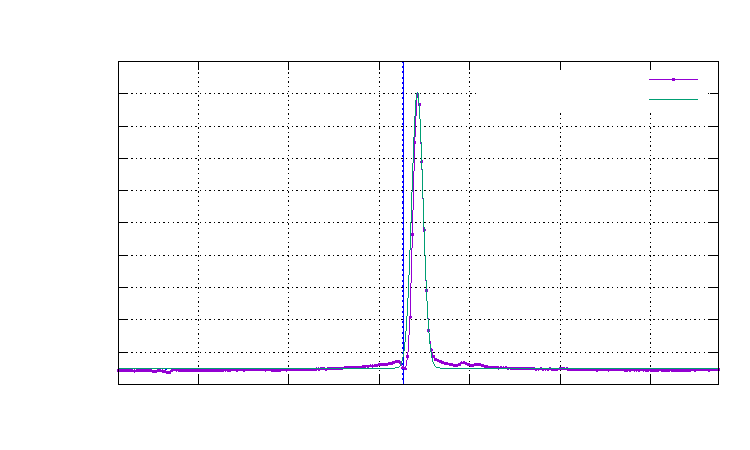
\includegraphics[width={360.00bp},height={216.00bp}]{P-Cygni_H_gauss}}%
    \gplfronttext
  \end{picture}%
\endgroup
}
  \caption{} \label{fig:pcH}
\end{figure}
\begin{figure}[h]
  \centering
  \resizebox{.5\textwidth}{!}{% GNUPLOT: LaTeX picture with Postscript
\begingroup
  \makeatletter
  \providecommand\color[2][]{%
    \GenericError{(gnuplot) \space\space\space\@spaces}{%
      Package color not loaded in conjunction with
      terminal option `colourtext'%
    }{See the gnuplot documentation for explanation.%
    }{Either use 'blacktext' in gnuplot or load the package
      color.sty in LaTeX.}%
    \renewcommand\color[2][]{}%
  }%
  \providecommand\includegraphics[2][]{%
    \GenericError{(gnuplot) \space\space\space\@spaces}{%
      Package graphicx or graphics not loaded%
    }{See the gnuplot documentation for explanation.%
    }{The gnuplot epslatex terminal needs graphicx.sty or graphics.sty.}%
    \renewcommand\includegraphics[2][]{}%
  }%
  \providecommand\rotatebox[2]{#2}%
  \@ifundefined{ifGPcolor}{%
    \newif\ifGPcolor
    \GPcolortrue
  }{}%
  \@ifundefined{ifGPblacktext}{%
    \newif\ifGPblacktext
    \GPblacktexttrue
  }{}%
  % define a \g@addto@macro without @ in the name:
  \let\gplgaddtomacro\g@addto@macro
  % define empty templates for all commands taking text:
  \gdef\gplbacktext{}%
  \gdef\gplfronttext{}%
  \makeatother
  \ifGPblacktext
    % no textcolor at all
    \def\colorrgb#1{}%
    \def\colorgray#1{}%
  \else
    % gray or color?
    \ifGPcolor
      \def\colorrgb#1{\color[rgb]{#1}}%
      \def\colorgray#1{\color[gray]{#1}}%
      \expandafter\def\csname LTw\endcsname{\color{white}}%
      \expandafter\def\csname LTb\endcsname{\color{black}}%
      \expandafter\def\csname LTa\endcsname{\color{black}}%
      \expandafter\def\csname LT0\endcsname{\color[rgb]{1,0,0}}%
      \expandafter\def\csname LT1\endcsname{\color[rgb]{0,1,0}}%
      \expandafter\def\csname LT2\endcsname{\color[rgb]{0,0,1}}%
      \expandafter\def\csname LT3\endcsname{\color[rgb]{1,0,1}}%
      \expandafter\def\csname LT4\endcsname{\color[rgb]{0,1,1}}%
      \expandafter\def\csname LT5\endcsname{\color[rgb]{1,1,0}}%
      \expandafter\def\csname LT6\endcsname{\color[rgb]{0,0,0}}%
      \expandafter\def\csname LT7\endcsname{\color[rgb]{1,0.3,0}}%
      \expandafter\def\csname LT8\endcsname{\color[rgb]{0.5,0.5,0.5}}%
    \else
      % gray
      \def\colorrgb#1{\color{black}}%
      \def\colorgray#1{\color[gray]{#1}}%
      \expandafter\def\csname LTw\endcsname{\color{white}}%
      \expandafter\def\csname LTb\endcsname{\color{black}}%
      \expandafter\def\csname LTa\endcsname{\color{black}}%
      \expandafter\def\csname LT0\endcsname{\color{black}}%
      \expandafter\def\csname LT1\endcsname{\color{black}}%
      \expandafter\def\csname LT2\endcsname{\color{black}}%
      \expandafter\def\csname LT3\endcsname{\color{black}}%
      \expandafter\def\csname LT4\endcsname{\color{black}}%
      \expandafter\def\csname LT5\endcsname{\color{black}}%
      \expandafter\def\csname LT6\endcsname{\color{black}}%
      \expandafter\def\csname LT7\endcsname{\color{black}}%
      \expandafter\def\csname LT8\endcsname{\color{black}}%
    \fi
  \fi
    \setlength{\unitlength}{0.0500bp}%
    \ifx\gptboxheight\undefined%
      \newlength{\gptboxheight}%
      \newlength{\gptboxwidth}%
      \newsavebox{\gptboxtext}%
    \fi%
    \setlength{\fboxrule}{0.5pt}%
    \setlength{\fboxsep}{1pt}%
    \definecolor{tbcol}{rgb}{1,1,1}%
\begin{picture}(7200.00,4320.00)%
    \gplgaddtomacro\gplbacktext{%
      \csname LTb\endcsname%%
      \put(1025,619){\makebox(0,0)[r]{\strut{}$30\cdot10^{3}$}}%
      \csname LTb\endcsname%%
      \put(1025,1006){\makebox(0,0)[r]{\strut{}$40\cdot10^{3}$}}%
      \csname LTb\endcsname%%
      \put(1025,1394){\makebox(0,0)[r]{\strut{}$50\cdot10^{3}$}}%
      \csname LTb\endcsname%%
      \put(1025,1781){\makebox(0,0)[r]{\strut{}$60\cdot10^{3}$}}%
      \csname LTb\endcsname%%
      \put(1025,2169){\makebox(0,0)[r]{\strut{}$70\cdot10^{3}$}}%
      \csname LTb\endcsname%%
      \put(1025,2556){\makebox(0,0)[r]{\strut{}$80\cdot10^{3}$}}%
      \csname LTb\endcsname%%
      \put(1025,2944){\makebox(0,0)[r]{\strut{}$90\cdot10^{3}$}}%
      \csname LTb\endcsname%%
      \put(1025,3331){\makebox(0,0)[r]{\strut{}$100\cdot10^{3}$}}%
      \csname LTb\endcsname%%
      \put(1025,3719){\makebox(0,0)[r]{\strut{}$110\cdot10^{3}$}}%
      \csname LTb\endcsname%%
      \put(1326,425){\makebox(0,0){\strut{}$666\cdot10^{-9}$}}%
      \csname LTb\endcsname%%
      \put(2786,425){\makebox(0,0){\strut{}$667\cdot10^{-9}$}}%
      \csname LTb\endcsname%%
      \put(4245,425){\makebox(0,0){\strut{}$668\cdot10^{-9}$}}%
      \csname LTb\endcsname%%
      \put(5705,425){\makebox(0,0){\strut{}$669\cdot10^{-9}$}}%
    }%
    \gplgaddtomacro\gplfronttext{%
      \csname LTb\endcsname%%
      \put(170,2169){\rotatebox{-270}{\makebox(0,0){\strut{}Amplitude$/\textrm{a.u.}$}}}%
      \csname LTb\endcsname%%
      \put(4004,135){\makebox(0,0){\strut{}Wellenlänge $\lambda/\SI{}{m}$}}%
      \csname LTb\endcsname%%
      \put(6123,3545){\makebox(0,0)[r]{\strut{}Datenpunkte}}%
      \csname LTb\endcsname%%
      \put(6123,3351){\makebox(0,0)[r]{\strut{}Anpassung $G_\text{f}(x)$}}%
      \csname LTb\endcsname%%
      \put(4004,4009){\makebox(0,0){\strut{}Spektrallinie von N2 mit $\chi^2/\textrm{ddof}=\SI{2.17E-01}{}$}}%
    }%
    \gplbacktext
    \put(0,0){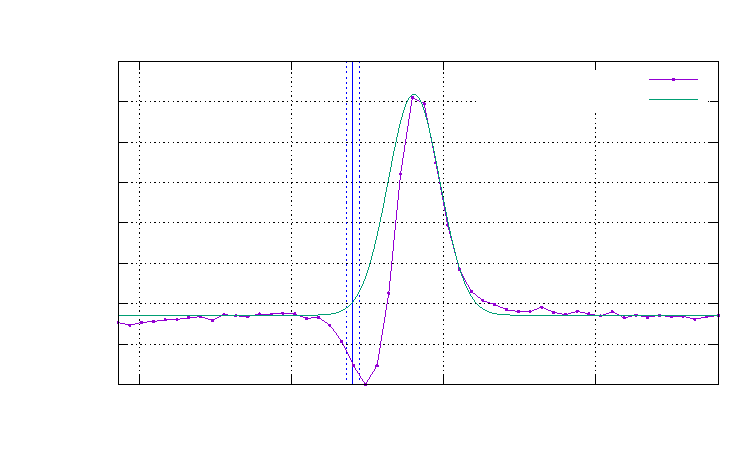
\includegraphics[width={360.00bp},height={216.00bp}]{P-Cygni_N2_gauss}}%
    \gplfronttext
  \end{picture}%
\endgroup
}
  \caption{} \label{fig:pcN2}
\end{figure}
\begin{figure}[h]
  \centering
  \resizebox{.5\textwidth}{!}{% GNUPLOT: LaTeX picture with Postscript
\begingroup
  \makeatletter
  \providecommand\color[2][]{%
    \GenericError{(gnuplot) \space\space\space\@spaces}{%
      Package color not loaded in conjunction with
      terminal option `colourtext'%
    }{See the gnuplot documentation for explanation.%
    }{Either use 'blacktext' in gnuplot or load the package
      color.sty in LaTeX.}%
    \renewcommand\color[2][]{}%
  }%
  \providecommand\includegraphics[2][]{%
    \GenericError{(gnuplot) \space\space\space\@spaces}{%
      Package graphicx or graphics not loaded%
    }{See the gnuplot documentation for explanation.%
    }{The gnuplot epslatex terminal needs graphicx.sty or graphics.sty.}%
    \renewcommand\includegraphics[2][]{}%
  }%
  \providecommand\rotatebox[2]{#2}%
  \@ifundefined{ifGPcolor}{%
    \newif\ifGPcolor
    \GPcolortrue
  }{}%
  \@ifundefined{ifGPblacktext}{%
    \newif\ifGPblacktext
    \GPblacktexttrue
  }{}%
  % define a \g@addto@macro without @ in the name:
  \let\gplgaddtomacro\g@addto@macro
  % define empty templates for all commands taking text:
  \gdef\gplbacktext{}%
  \gdef\gplfronttext{}%
  \makeatother
  \ifGPblacktext
    % no textcolor at all
    \def\colorrgb#1{}%
    \def\colorgray#1{}%
  \else
    % gray or color?
    \ifGPcolor
      \def\colorrgb#1{\color[rgb]{#1}}%
      \def\colorgray#1{\color[gray]{#1}}%
      \expandafter\def\csname LTw\endcsname{\color{white}}%
      \expandafter\def\csname LTb\endcsname{\color{black}}%
      \expandafter\def\csname LTa\endcsname{\color{black}}%
      \expandafter\def\csname LT0\endcsname{\color[rgb]{1,0,0}}%
      \expandafter\def\csname LT1\endcsname{\color[rgb]{0,1,0}}%
      \expandafter\def\csname LT2\endcsname{\color[rgb]{0,0,1}}%
      \expandafter\def\csname LT3\endcsname{\color[rgb]{1,0,1}}%
      \expandafter\def\csname LT4\endcsname{\color[rgb]{0,1,1}}%
      \expandafter\def\csname LT5\endcsname{\color[rgb]{1,1,0}}%
      \expandafter\def\csname LT6\endcsname{\color[rgb]{0,0,0}}%
      \expandafter\def\csname LT7\endcsname{\color[rgb]{1,0.3,0}}%
      \expandafter\def\csname LT8\endcsname{\color[rgb]{0.5,0.5,0.5}}%
    \else
      % gray
      \def\colorrgb#1{\color{black}}%
      \def\colorgray#1{\color[gray]{#1}}%
      \expandafter\def\csname LTw\endcsname{\color{white}}%
      \expandafter\def\csname LTb\endcsname{\color{black}}%
      \expandafter\def\csname LTa\endcsname{\color{black}}%
      \expandafter\def\csname LT0\endcsname{\color{black}}%
      \expandafter\def\csname LT1\endcsname{\color{black}}%
      \expandafter\def\csname LT2\endcsname{\color{black}}%
      \expandafter\def\csname LT3\endcsname{\color{black}}%
      \expandafter\def\csname LT4\endcsname{\color{black}}%
      \expandafter\def\csname LT5\endcsname{\color{black}}%
      \expandafter\def\csname LT6\endcsname{\color{black}}%
      \expandafter\def\csname LT7\endcsname{\color{black}}%
      \expandafter\def\csname LT8\endcsname{\color{black}}%
    \fi
  \fi
    \setlength{\unitlength}{0.0500bp}%
    \ifx\gptboxheight\undefined%
      \newlength{\gptboxheight}%
      \newlength{\gptboxwidth}%
      \newsavebox{\gptboxtext}%
    \fi%
    \setlength{\fboxrule}{0.5pt}%
    \setlength{\fboxsep}{1pt}%
    \definecolor{tbcol}{rgb}{1,1,1}%
\begin{picture}(7200.00,4320.00)%
    \gplgaddtomacro\gplbacktext{%
      \csname LTb\endcsname%%
      \put(927,619){\makebox(0,0)[r]{\strut{}$40\cdot10^{3}$}}%
      \csname LTb\endcsname%%
      \put(927,963){\makebox(0,0)[r]{\strut{}$42\cdot10^{3}$}}%
      \csname LTb\endcsname%%
      \put(927,1308){\makebox(0,0)[r]{\strut{}$44\cdot10^{3}$}}%
      \csname LTb\endcsname%%
      \put(927,1652){\makebox(0,0)[r]{\strut{}$46\cdot10^{3}$}}%
      \csname LTb\endcsname%%
      \put(927,1997){\makebox(0,0)[r]{\strut{}$48\cdot10^{3}$}}%
      \csname LTb\endcsname%%
      \put(927,2341){\makebox(0,0)[r]{\strut{}$50\cdot10^{3}$}}%
      \csname LTb\endcsname%%
      \put(927,2686){\makebox(0,0)[r]{\strut{}$52\cdot10^{3}$}}%
      \csname LTb\endcsname%%
      \put(927,3030){\makebox(0,0)[r]{\strut{}$54\cdot10^{3}$}}%
      \csname LTb\endcsname%%
      \put(927,3374){\makebox(0,0)[r]{\strut{}$56\cdot10^{3}$}}%
      \csname LTb\endcsname%%
      \put(927,3719){\makebox(0,0)[r]{\strut{}$58\cdot10^{3}$}}%
      \csname LTb\endcsname%%
      \put(1025,425){\makebox(0,0){\strut{}$632\cdot10^{-9}$}}%
      \csname LTb\endcsname%%
      \put(1758,425){\makebox(0,0){\strut{}$633\cdot10^{-9}$}}%
      \csname LTb\endcsname%%
      \put(2490,425){\makebox(0,0){\strut{}$634\cdot10^{-9}$}}%
      \csname LTb\endcsname%%
      \put(3223,425){\makebox(0,0){\strut{}$635\cdot10^{-9}$}}%
      \csname LTb\endcsname%%
      \put(3955,425){\makebox(0,0){\strut{}$636\cdot10^{-9}$}}%
      \csname LTb\endcsname%%
      \put(4688,425){\makebox(0,0){\strut{}$637\cdot10^{-9}$}}%
      \csname LTb\endcsname%%
      \put(5421,425){\makebox(0,0){\strut{}$638\cdot10^{-9}$}}%
      \csname LTb\endcsname%%
      \put(6153,425){\makebox(0,0){\strut{}$639\cdot10^{-9}$}}%
      \csname LTb\endcsname%%
      \put(6886,425){\makebox(0,0){\strut{}$640\cdot10^{-9}$}}%
    }%
    \gplgaddtomacro\gplfronttext{%
      \csname LTb\endcsname%%
      \put(170,2169){\rotatebox{-270}{\makebox(0,0){\strut{}Amplitude$/\textrm{a.u.}$}}}%
      \csname LTb\endcsname%%
      \put(3955,135){\makebox(0,0){\strut{}Wellenlänge $\lambda/\SI{}{m}$}}%
      \csname LTb\endcsname%%
      \put(6123,3545){\makebox(0,0)[r]{\strut{}Datenpunkte}}%
      \csname LTb\endcsname%%
      \put(6123,3351){\makebox(0,0)[r]{\strut{}Anpassung $G_\text{f}(x)$}}%
      \csname LTb\endcsname%%
      \put(3955,4009){\makebox(0,0){\strut{}Doublet von Si3 mit $\chi^2/\textrm{ddof}=\SI{5.51E-01}{}$}}%
    }%
    \gplbacktext
    \put(0,0){\includegraphics[width={360.00bp},height={216.00bp}]{P-Cygni_Si3_doublet}}%
    \gplfronttext
  \end{picture}%
\endgroup
}
  \caption{} \label{fig:pcSi3}
\end{figure}
\begin{figure}[t]
  \centering
  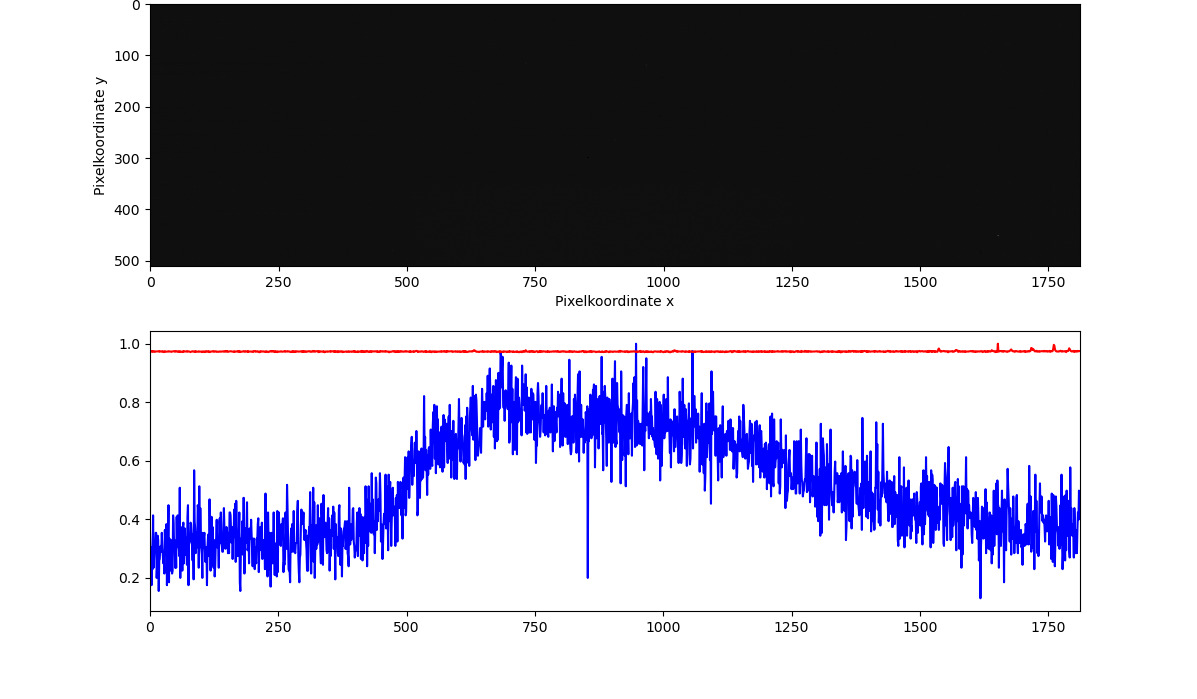
\includegraphics[width=.5\textwidth]{HD32630_beob.jpeg}
  \caption{Analyse des selbst aufgenommenen Spektrums von HD32630 mit nEDAR.} \label{fig:beob_hd32630}
\end{figure}
\begin{figure}[t]
  \centering
  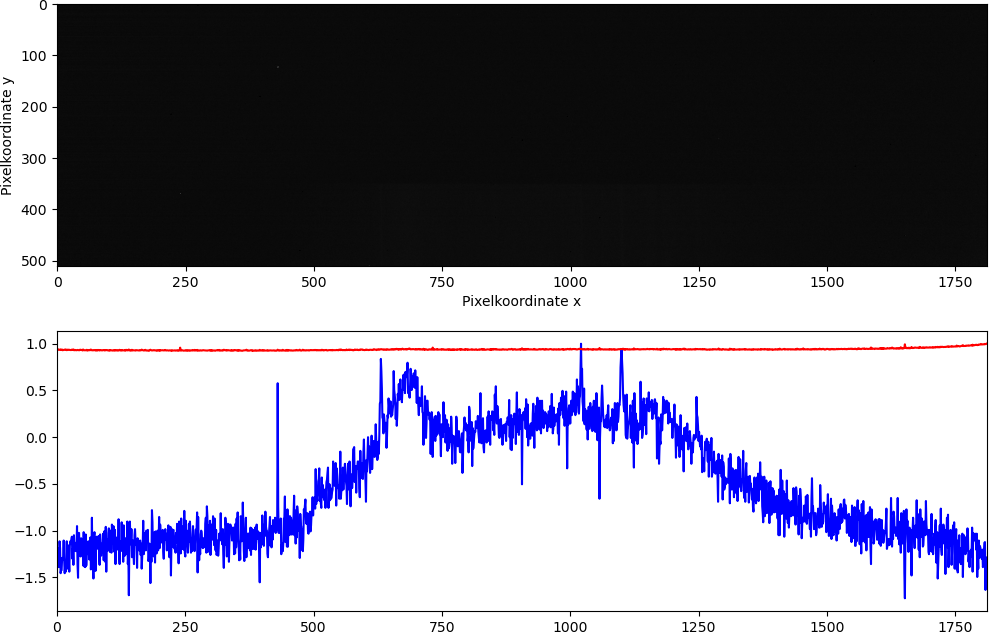
\includegraphics[width=.5\textwidth]{eigenes_spektrum_pcygni.png}
  \caption{Analyse des selbst aufgenommenen Spektrums von P Cygni mit nEDAR.} \label{fig:beob_pcygni}
\end{figure}
\begin{figure}[t]
  \centering
  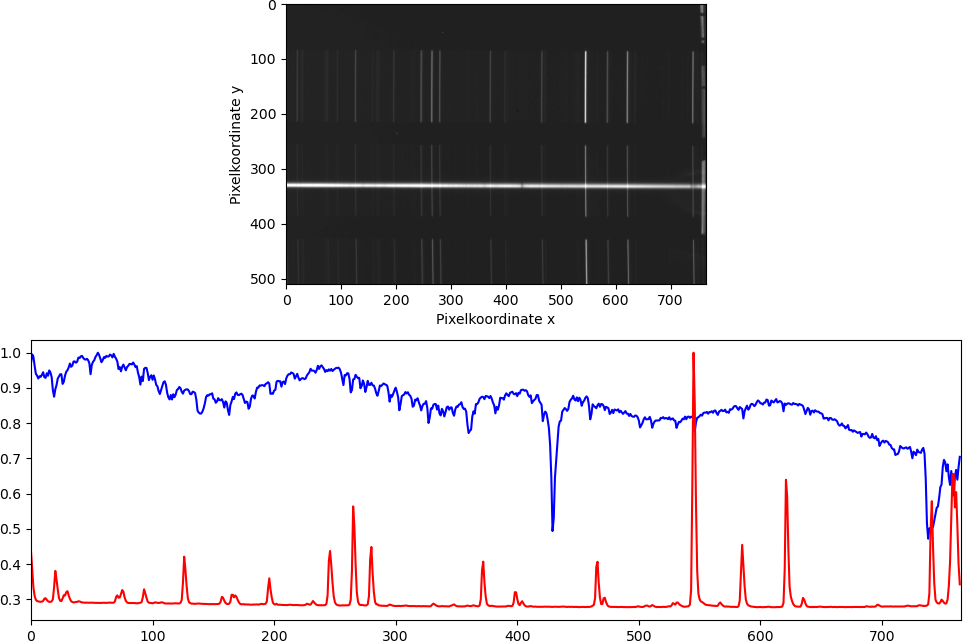
\includegraphics[width=.5\textwidth]{gestellter_stern_hd109358.png}
  \caption{Analyse der gestellten Daten von P Cygni mit nEDAR.} \label{fig:bereit_pcygni}
\end{figure}


\end{document}
